\begin{figure*}
\centering
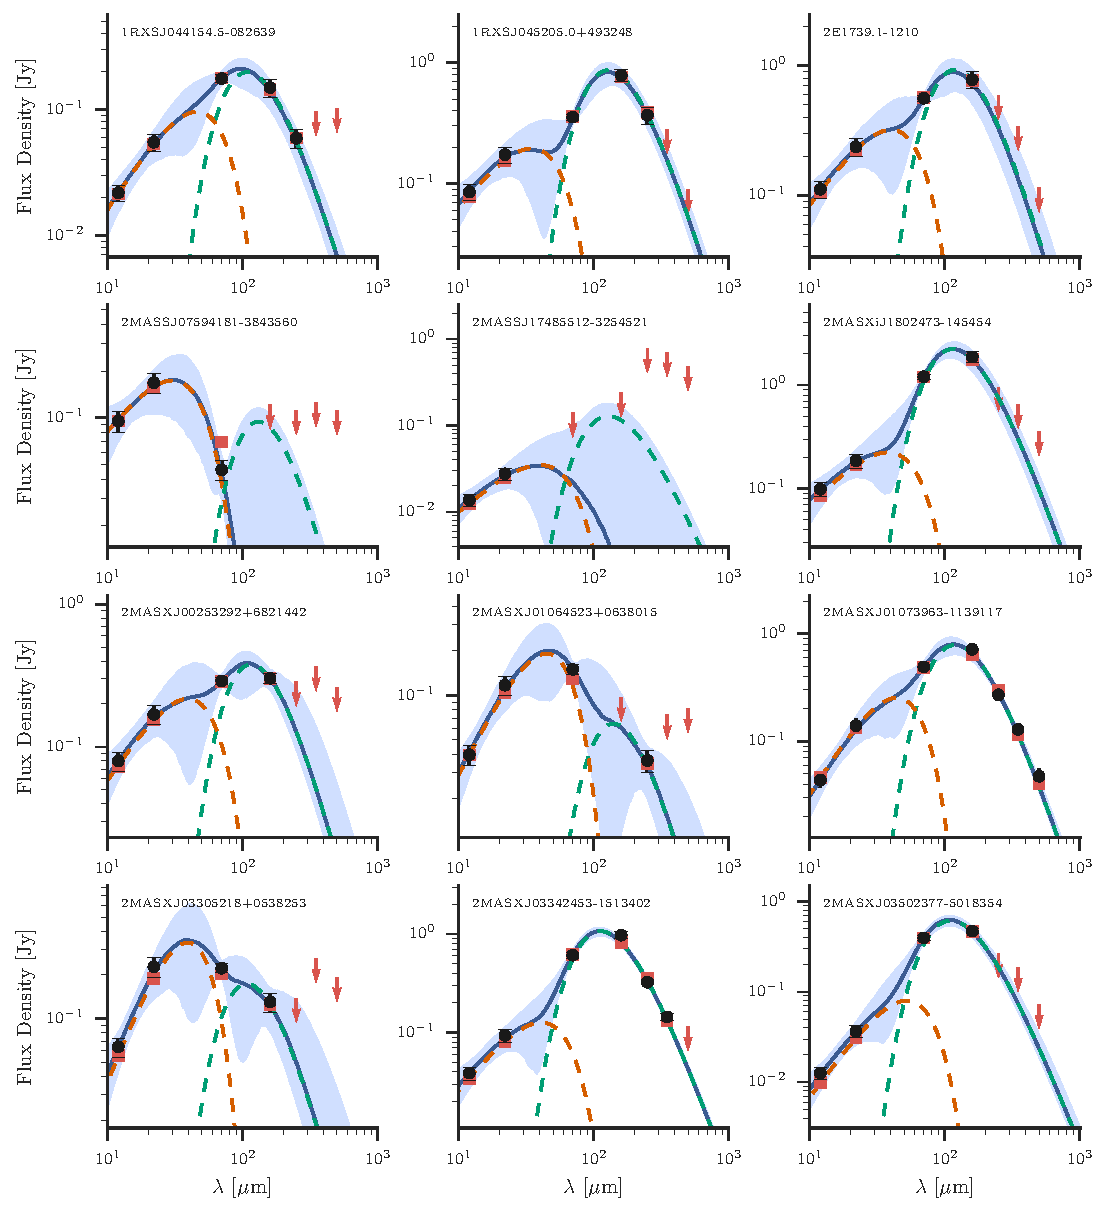
\includegraphics[width=\textwidth]{figures/sedfig1}
\caption{12--500 \micron{} SEDs for all of the \herschel-BAT sample. Black points plot the observed flux densities with open red circles indicating 5$\sigma$ upper limits. The solid blue line and shaded region shows the best-fit C12 model with a 95 percent confidence interval. The red squares are the model flux densities after convolving the best-fit model SED with each instrument's transmission curve. The orange and green dashed lines show the best-fit PL and MBB components, respectively. \label{fig:seds}}
\end{figure*}

\begin{figure*}
\centering
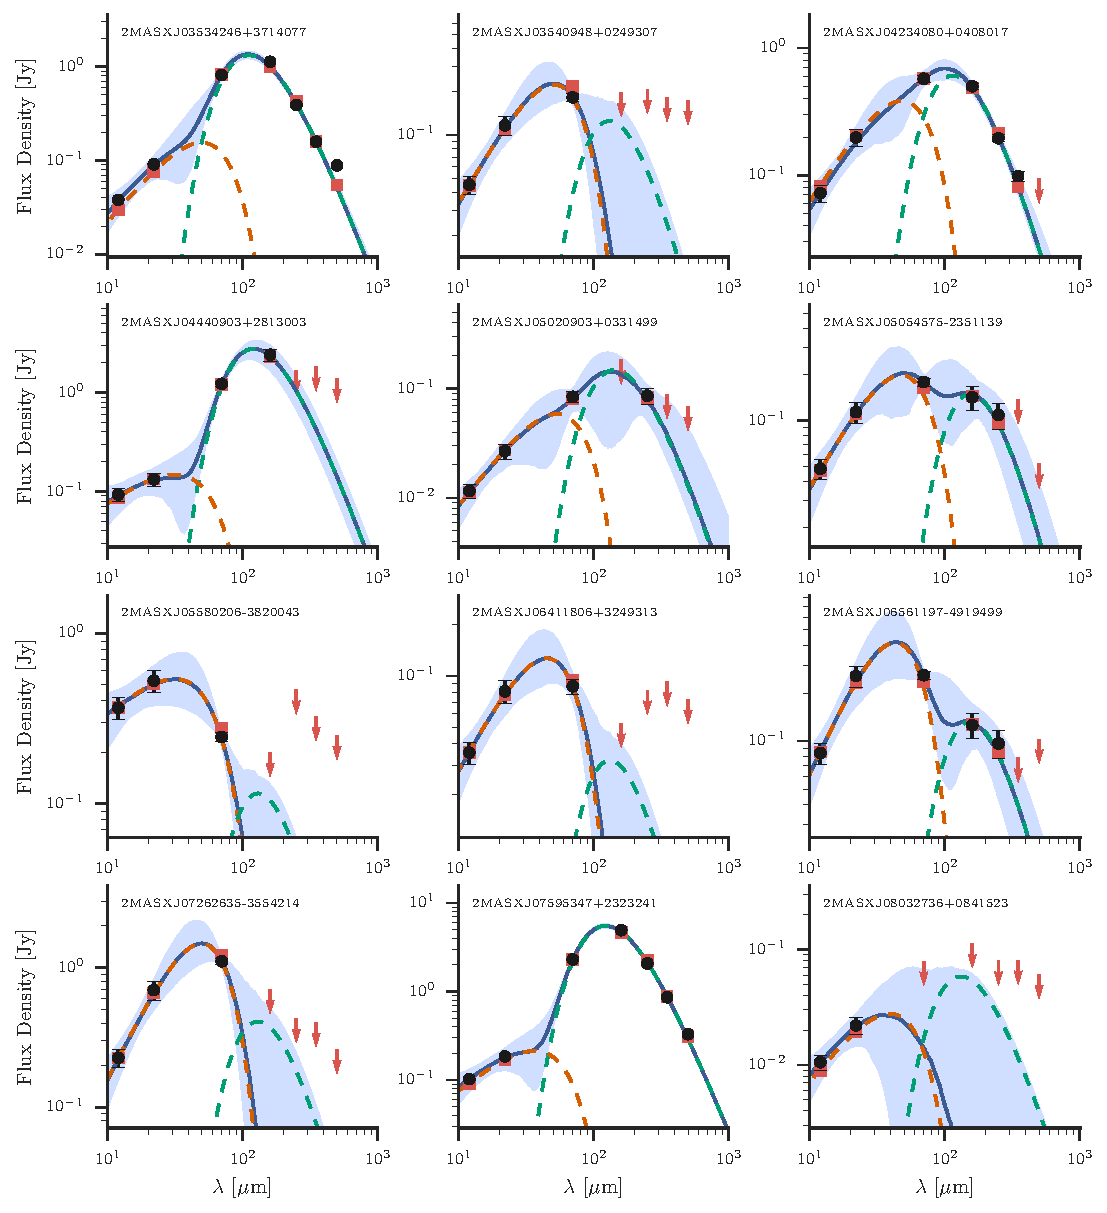
\includegraphics[width=\textwidth]{figures/sedfig2}
\caption{}
\end{figure*}

\begin{figure*}
\centering
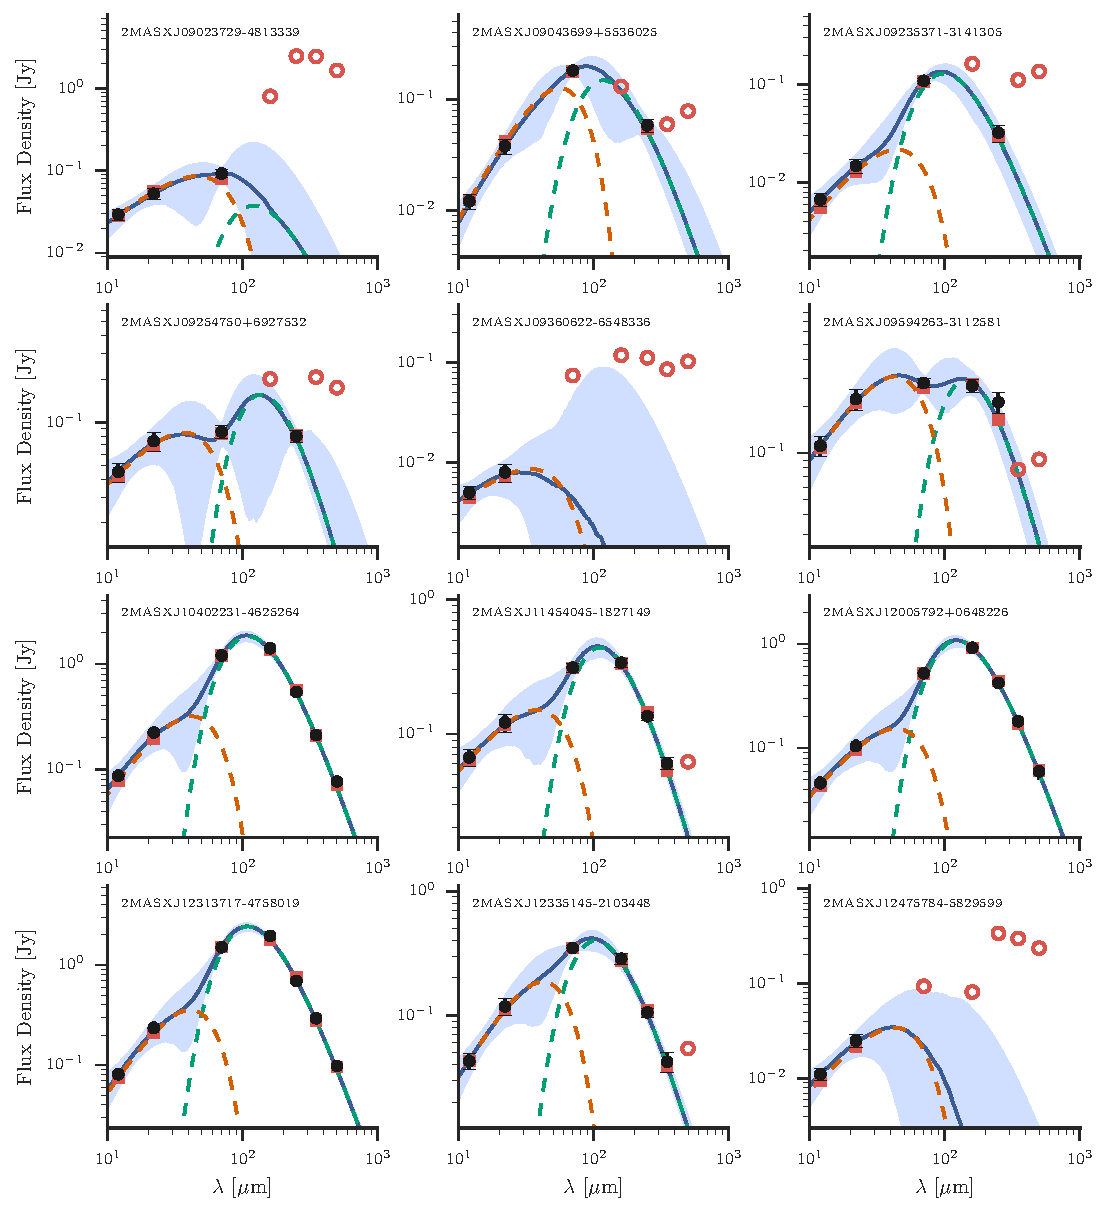
\includegraphics[width=\textwidth]{figures/sedfig3}
\caption{}
\end{figure*}

\begin{figure*}
\centering
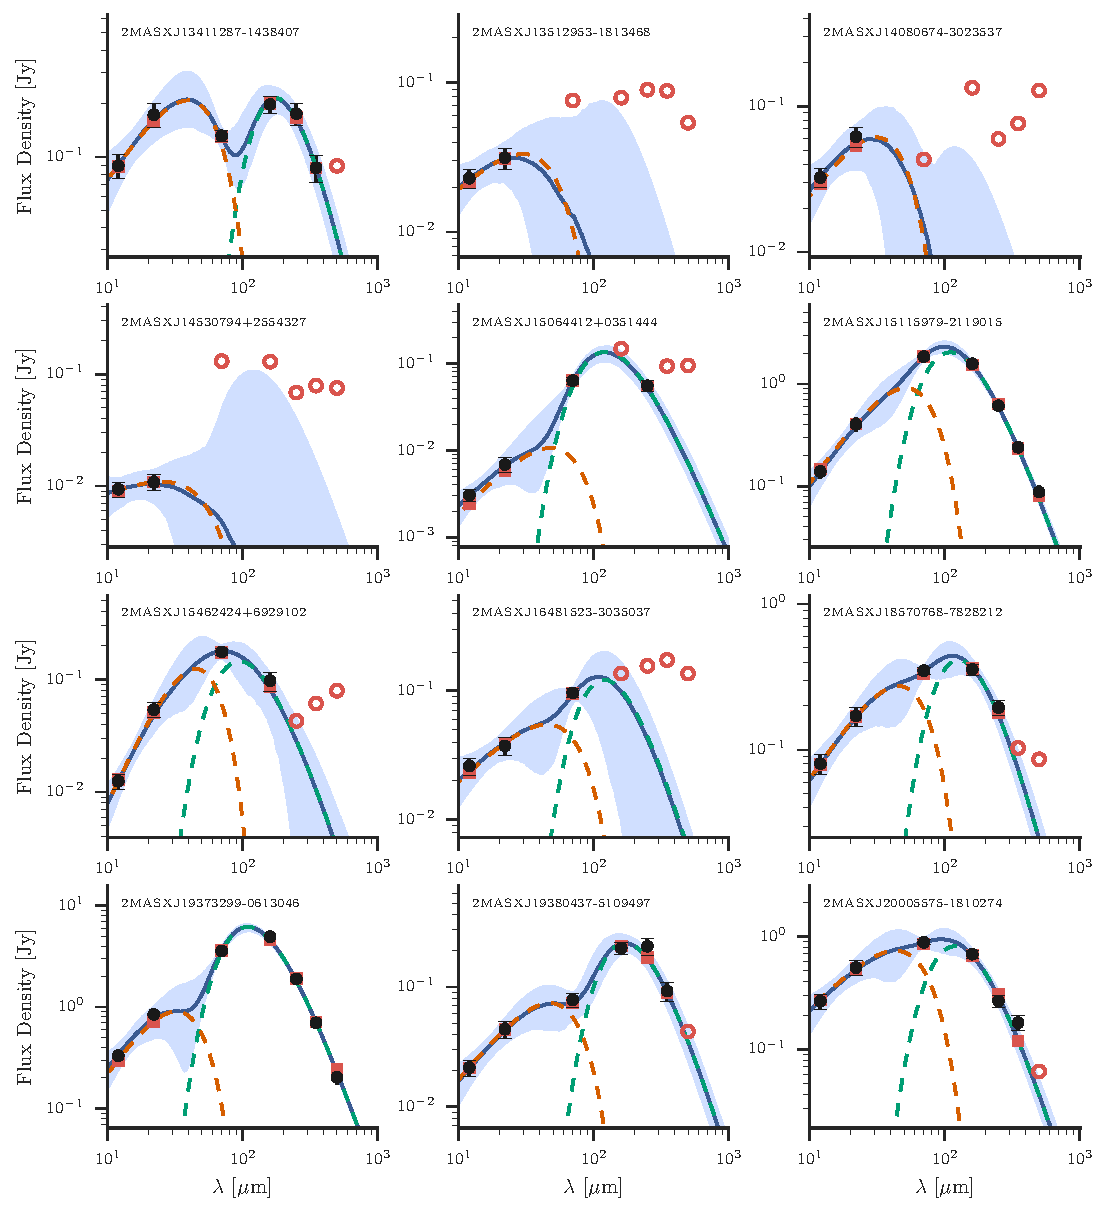
\includegraphics[width=\textwidth]{figures/sedfig4}
\caption{}
\end{figure*}

\begin{figure*}
\centering
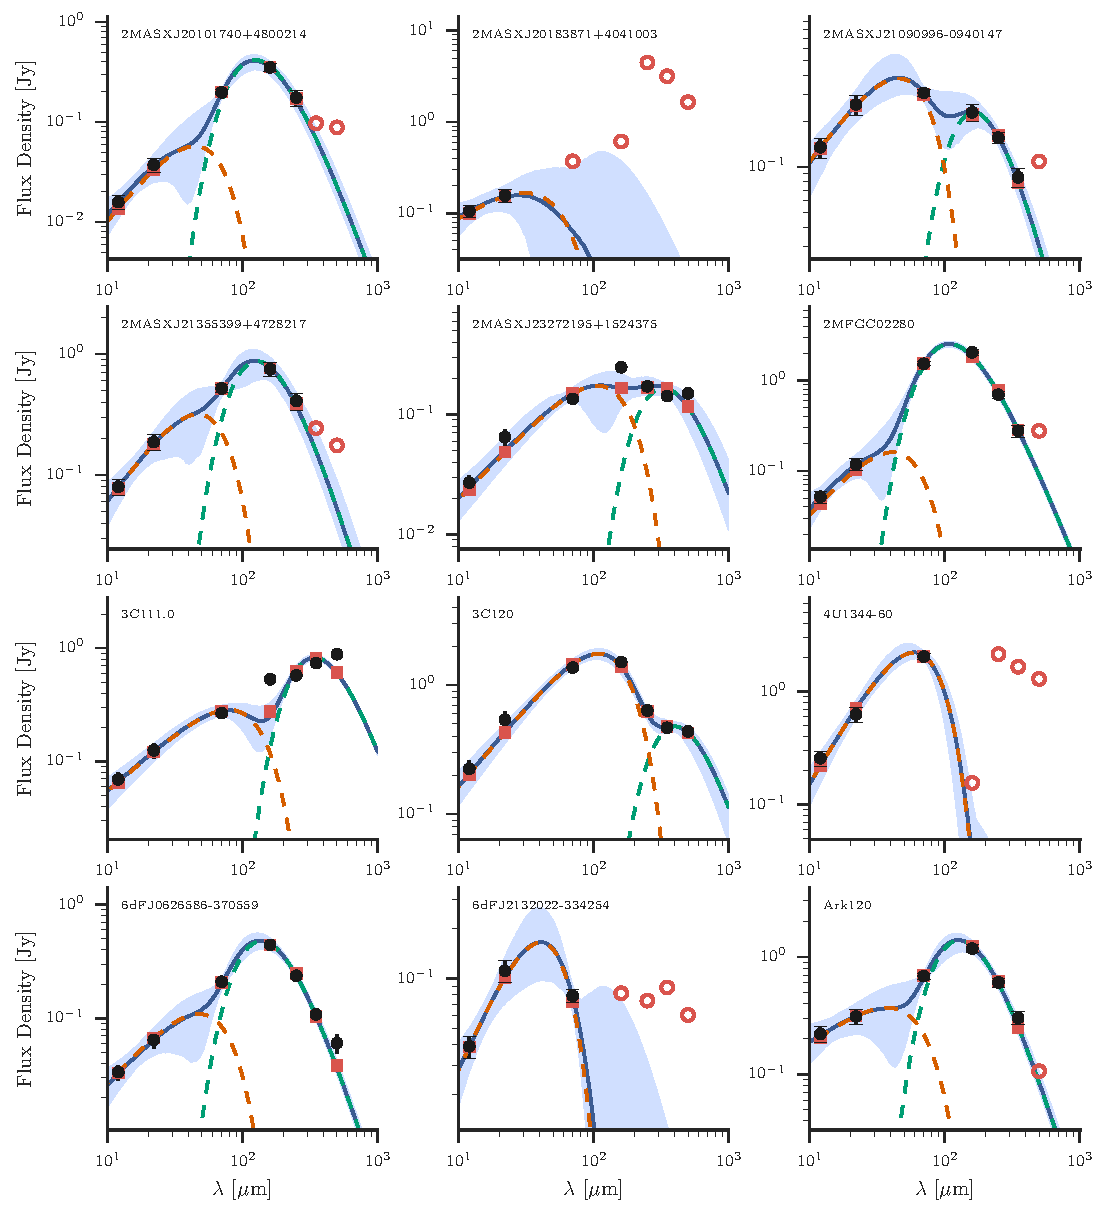
\includegraphics[width=\textwidth]{figures/sedfig5}
\caption{}
\end{figure*}

\begin{figure*}
\centering
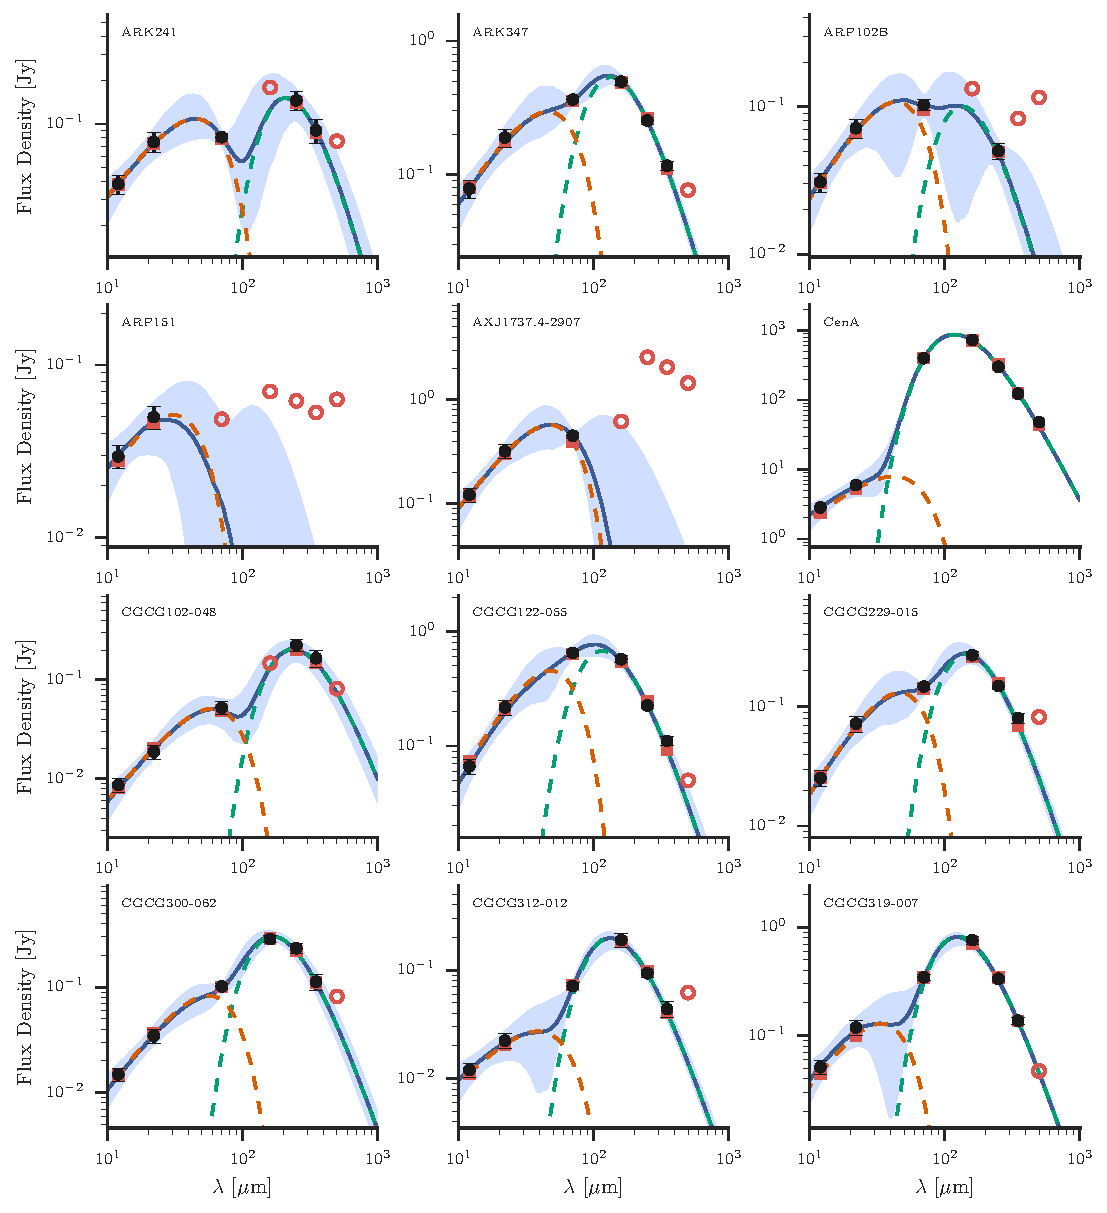
\includegraphics[width=\textwidth]{figures/sedfig6}
\caption{}
\end{figure*}

\begin{figure*}
\centering
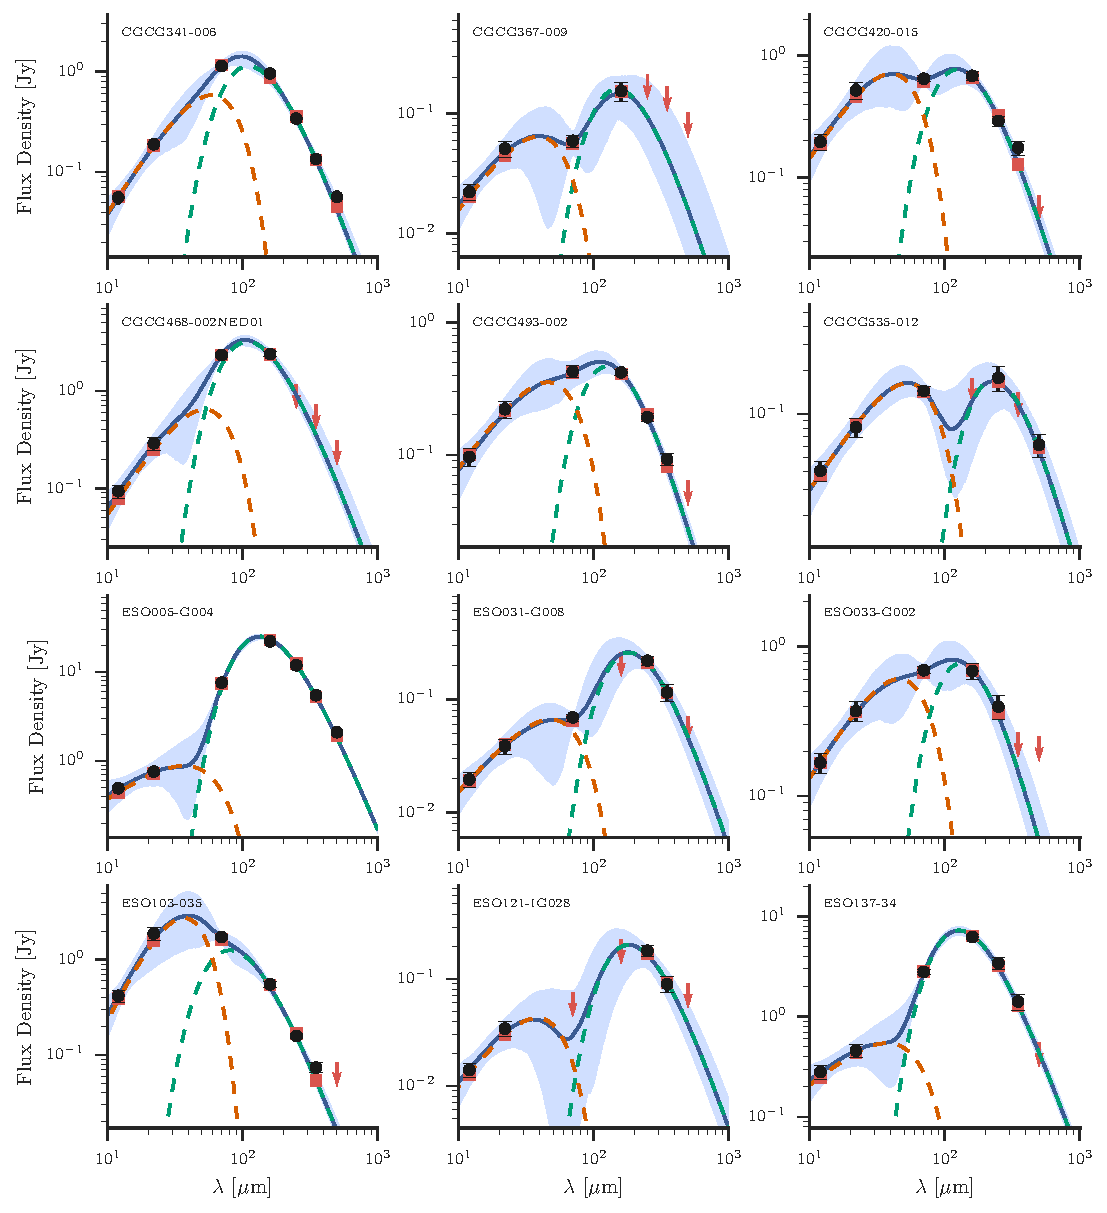
\includegraphics[width=\textwidth]{figures/sedfig7}
\caption{}
\end{figure*}

\begin{figure*}
\centering
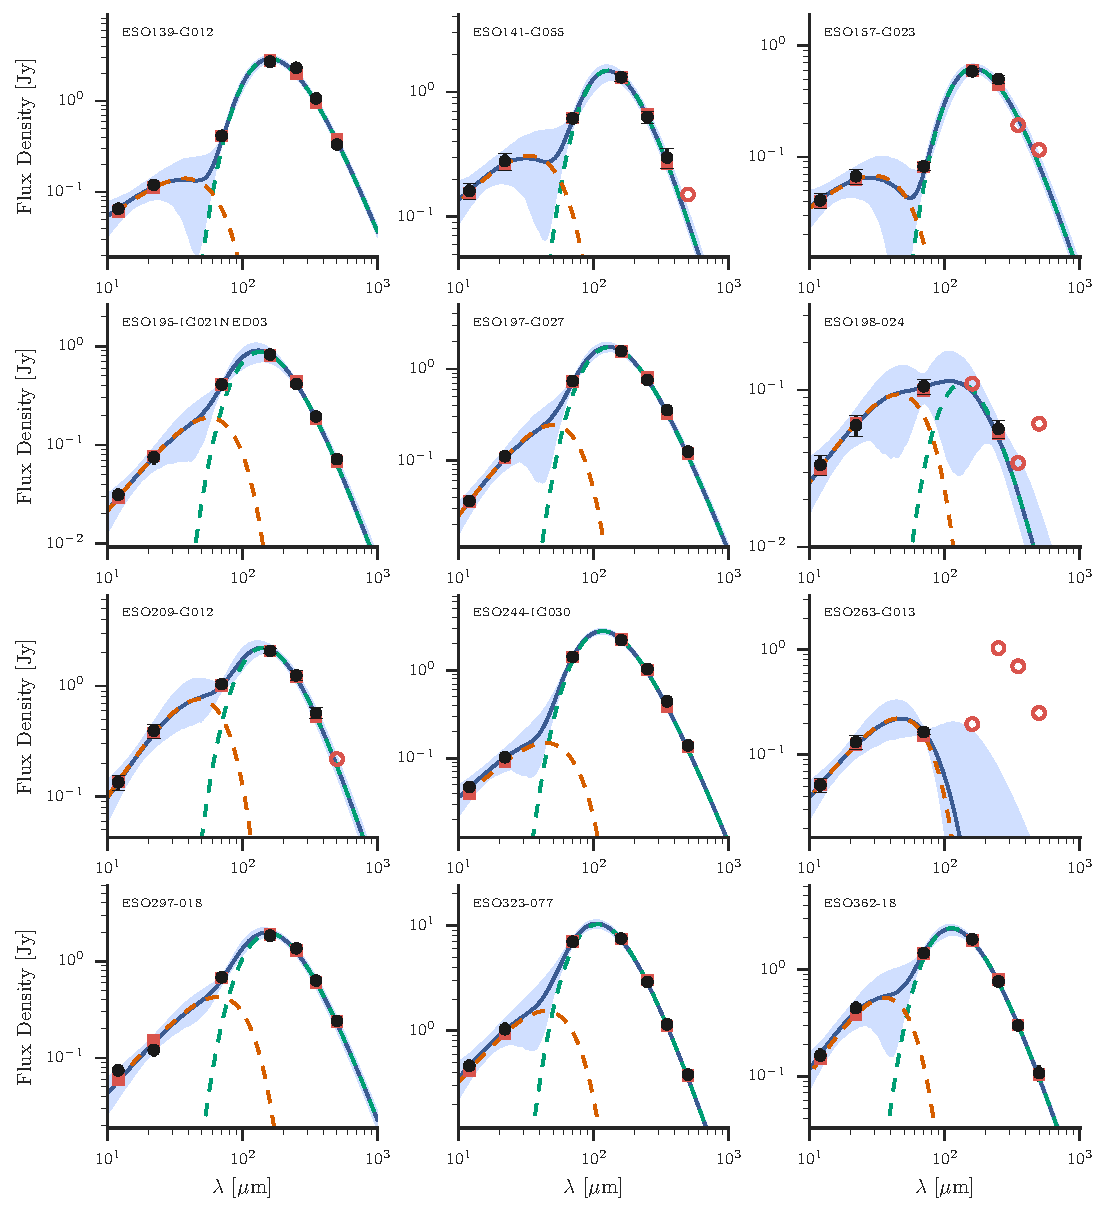
\includegraphics[width=\textwidth]{figures/sedfig8}
\caption{}
\end{figure*}

\begin{figure*}
\centering
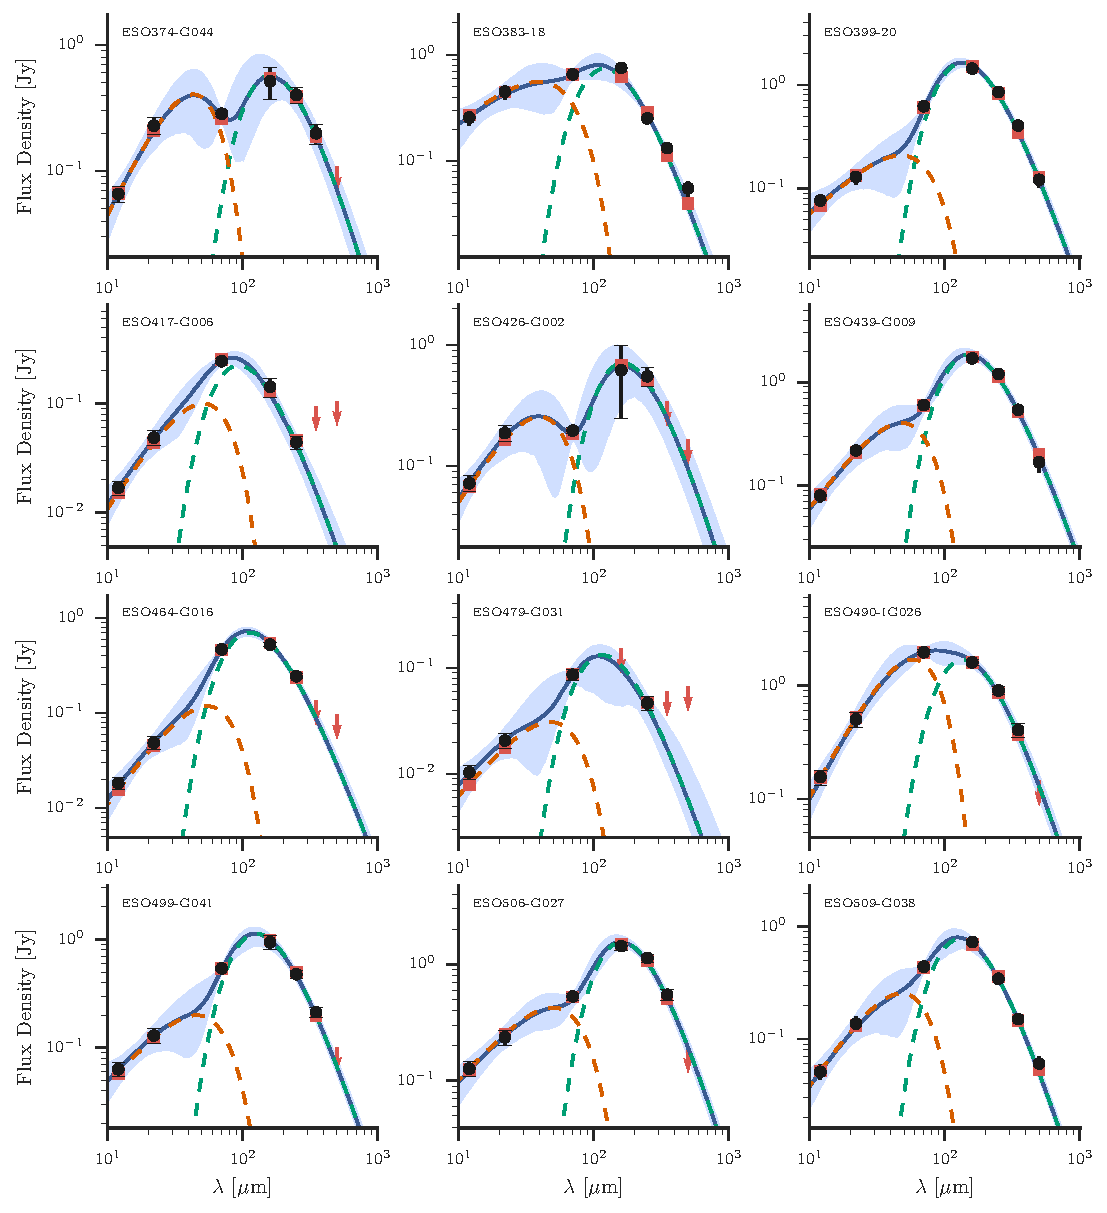
\includegraphics[width=\textwidth]{figures/sedfig9}
\caption{}
\end{figure*}

\begin{figure*}
\centering
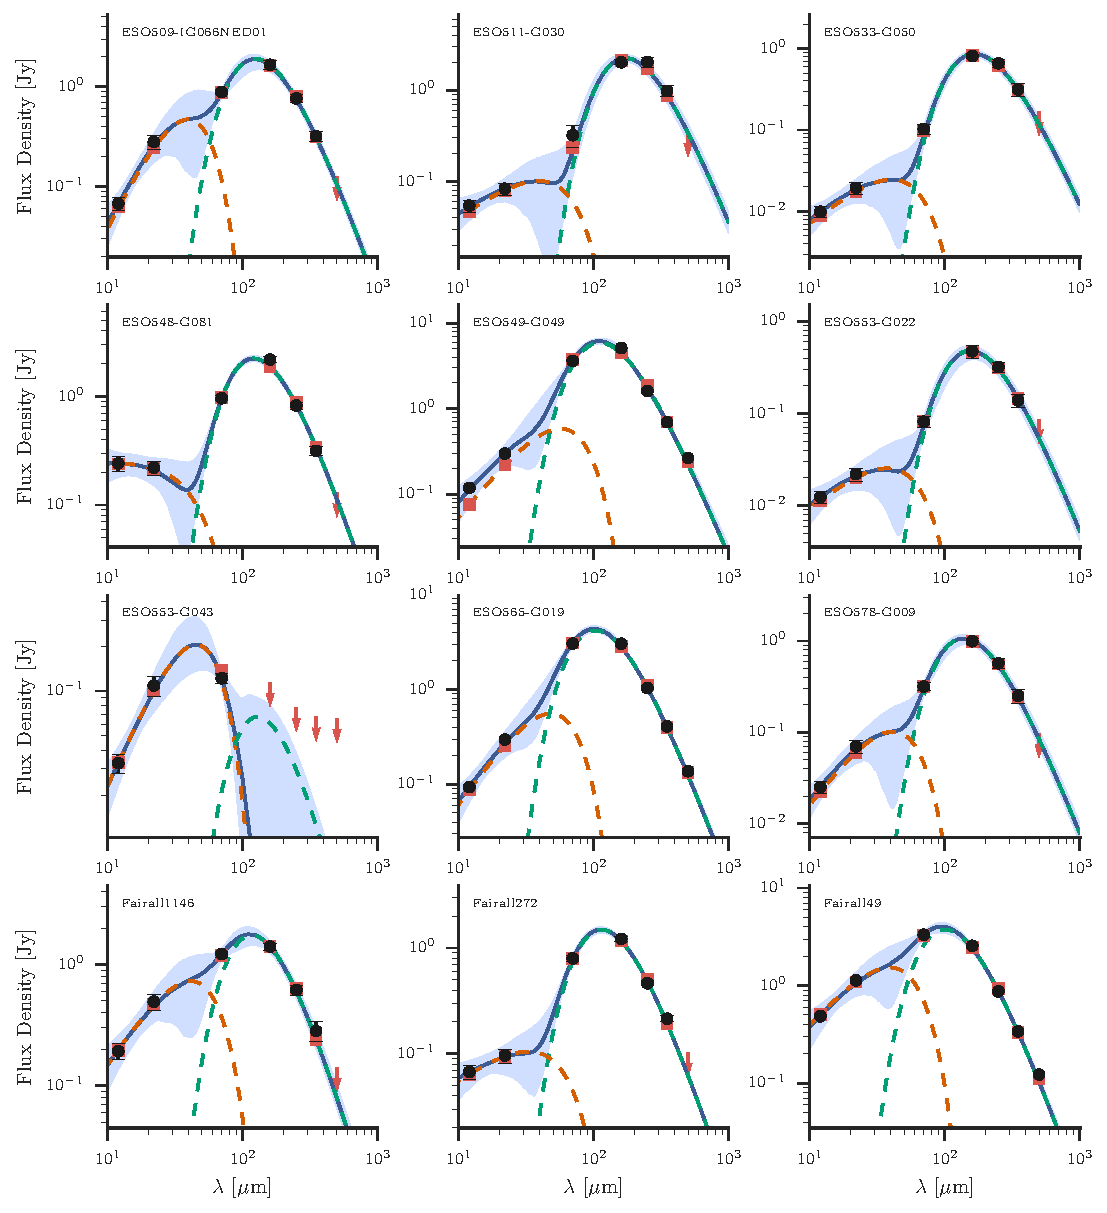
\includegraphics[width=\textwidth]{figures/sedfig10}
\caption{}
\end{figure*}

\begin{figure*}
\centering
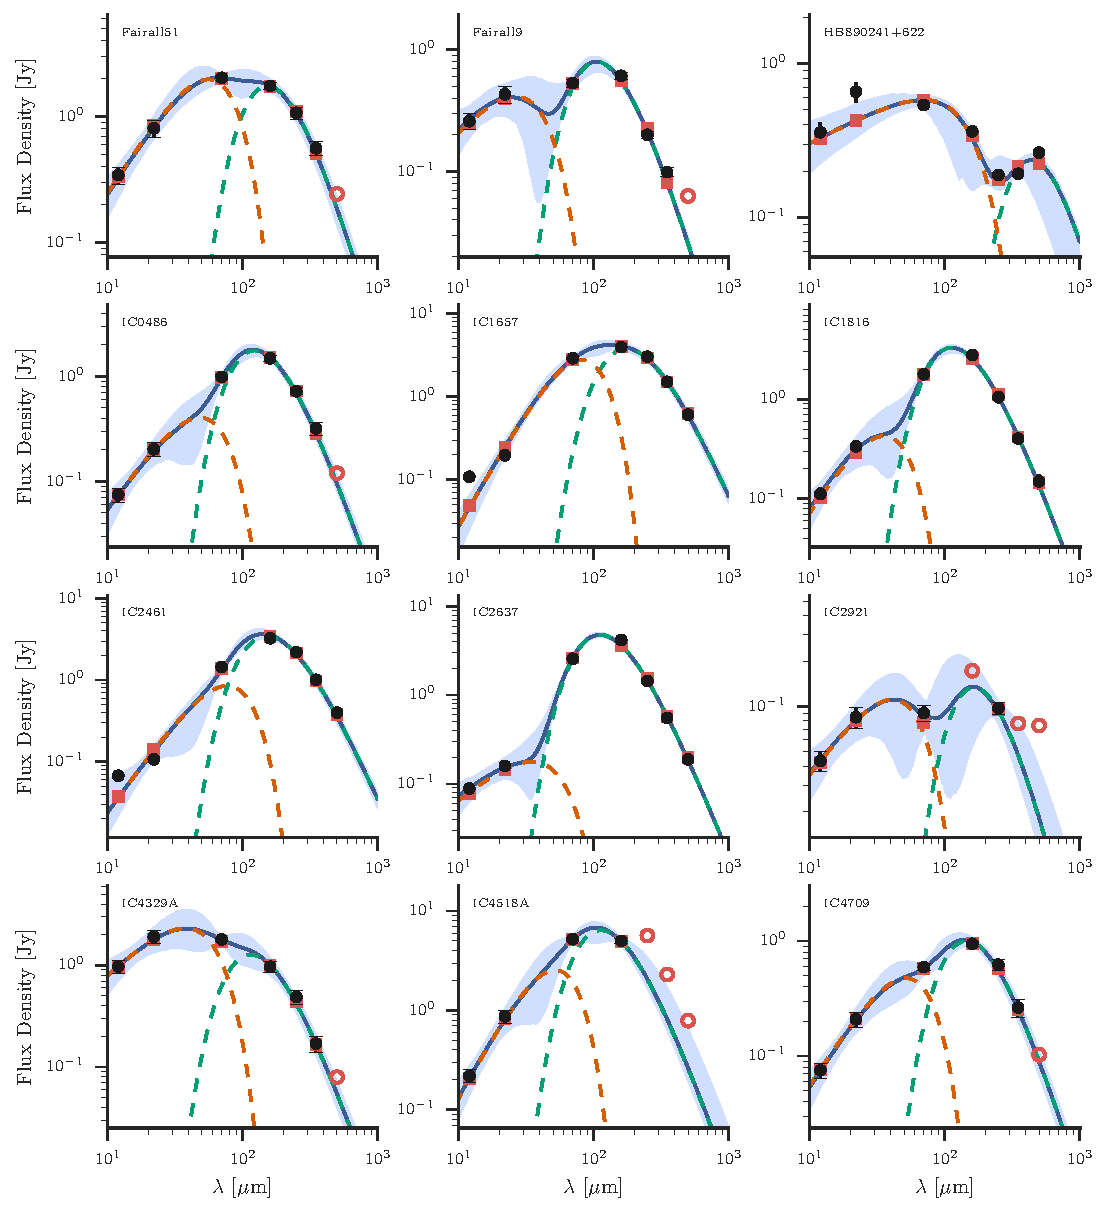
\includegraphics[width=\textwidth]{figures/sedfig11}
\caption{}
\end{figure*}

\begin{figure*}
\centering
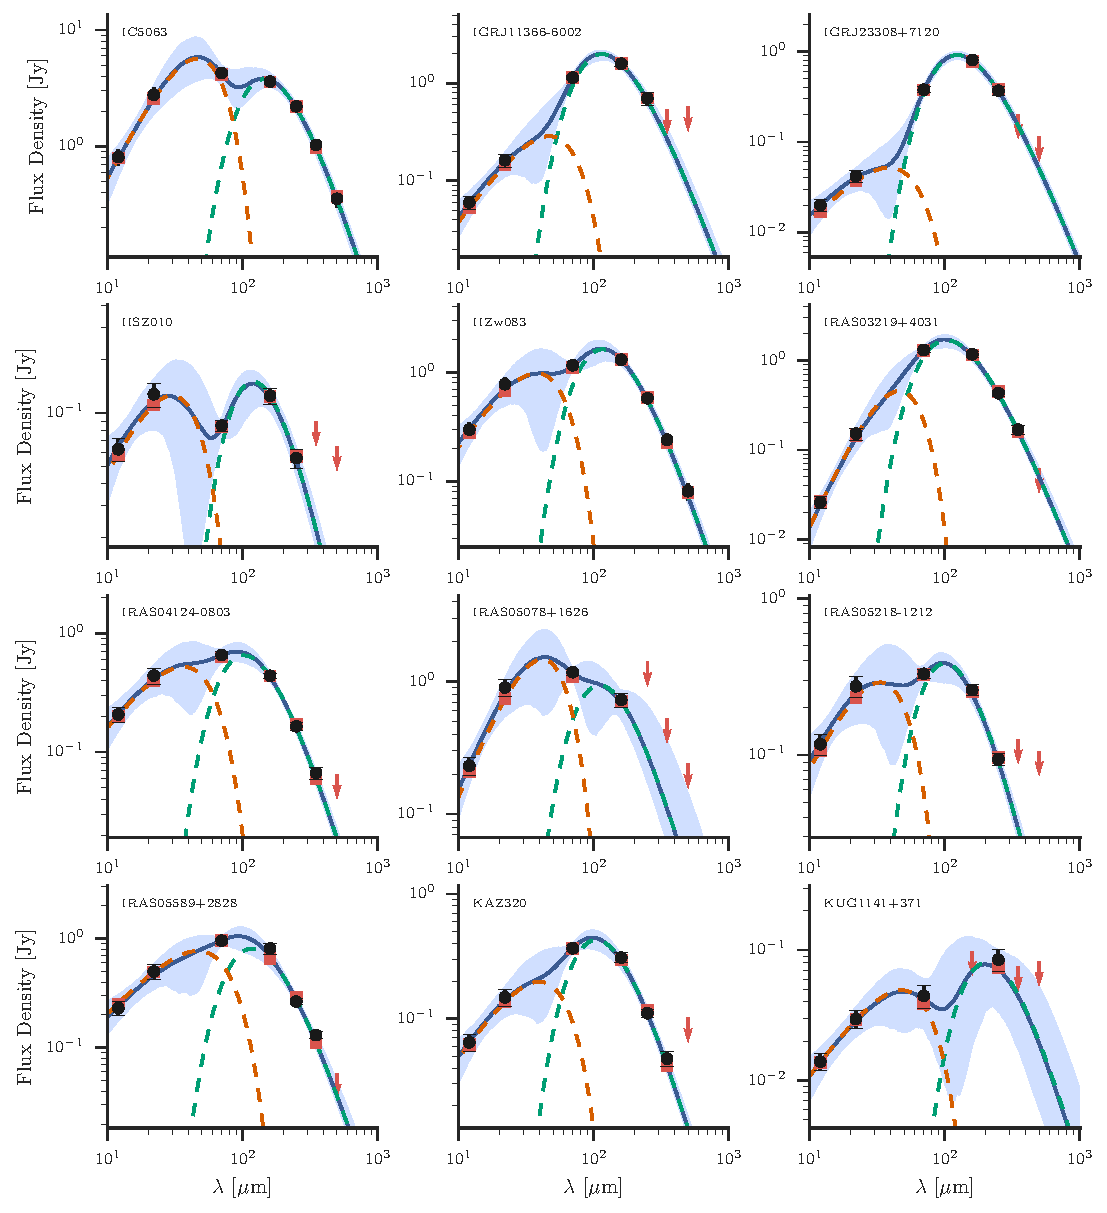
\includegraphics[width=\textwidth]{figures/sedfig12}
\caption{}
\end{figure*}

\begin{figure*}
\centering
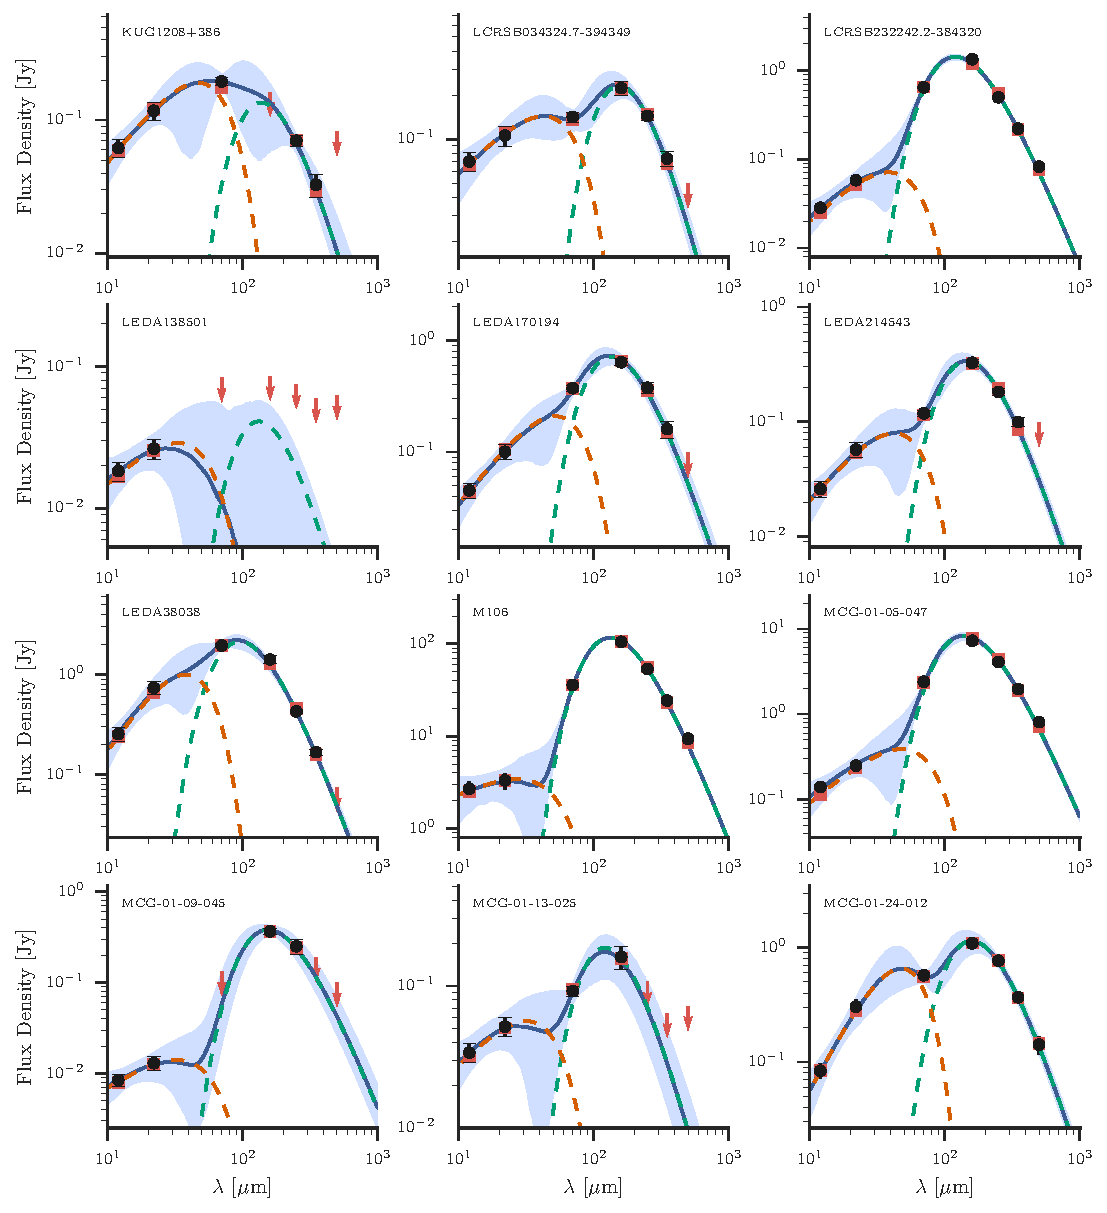
\includegraphics[width=\textwidth]{figures/sedfig13}
\caption{}
\end{figure*}

\begin{figure*}
\centering
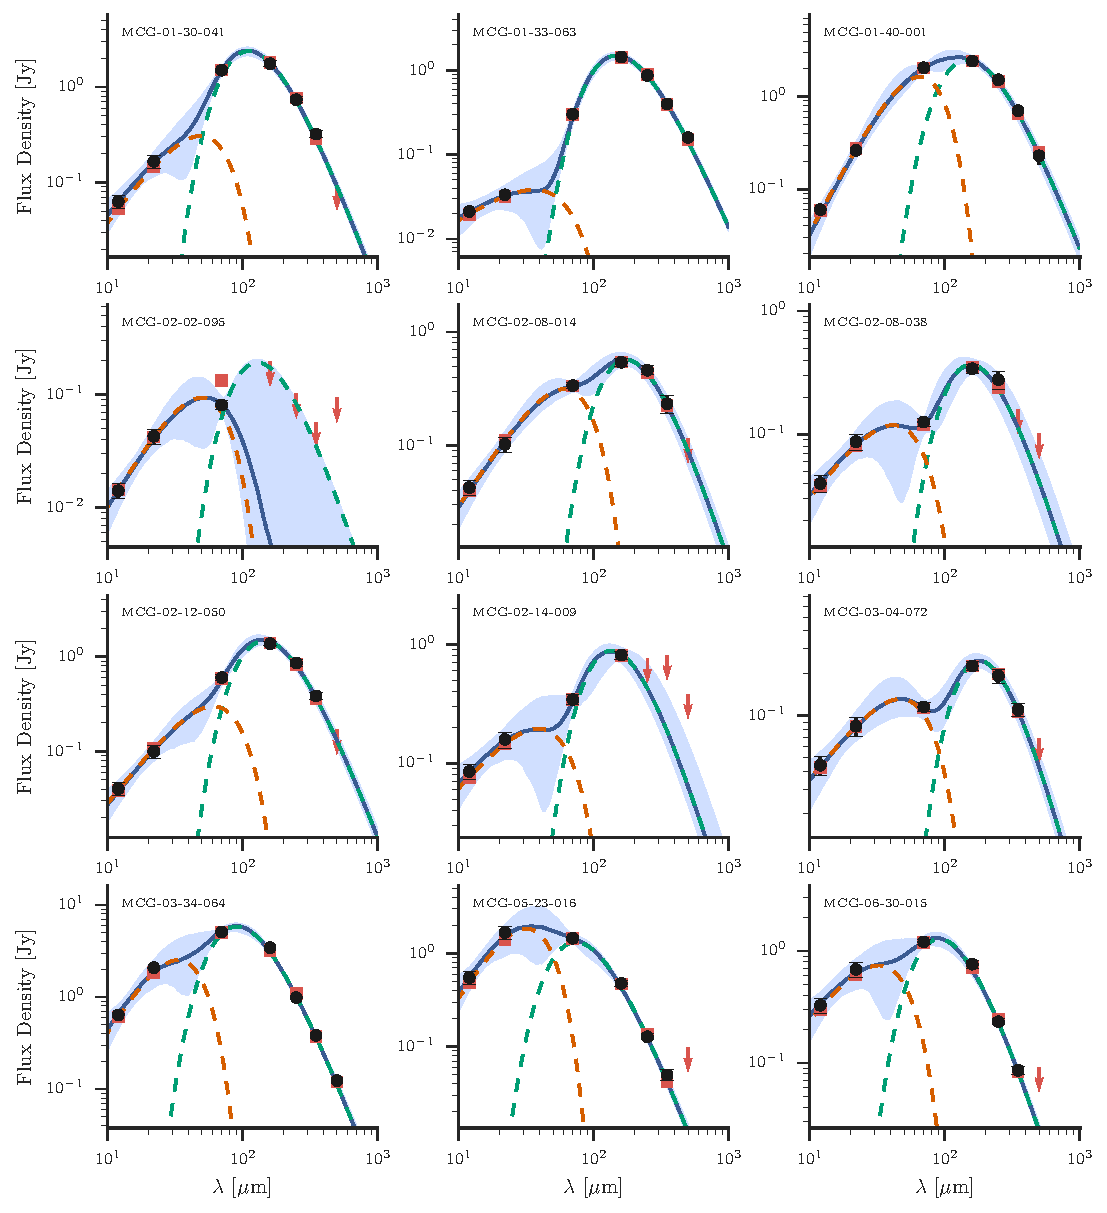
\includegraphics[width=\textwidth]{figures/sedfig14}
\caption{}
\end{figure*}

\begin{figure*}
\centering
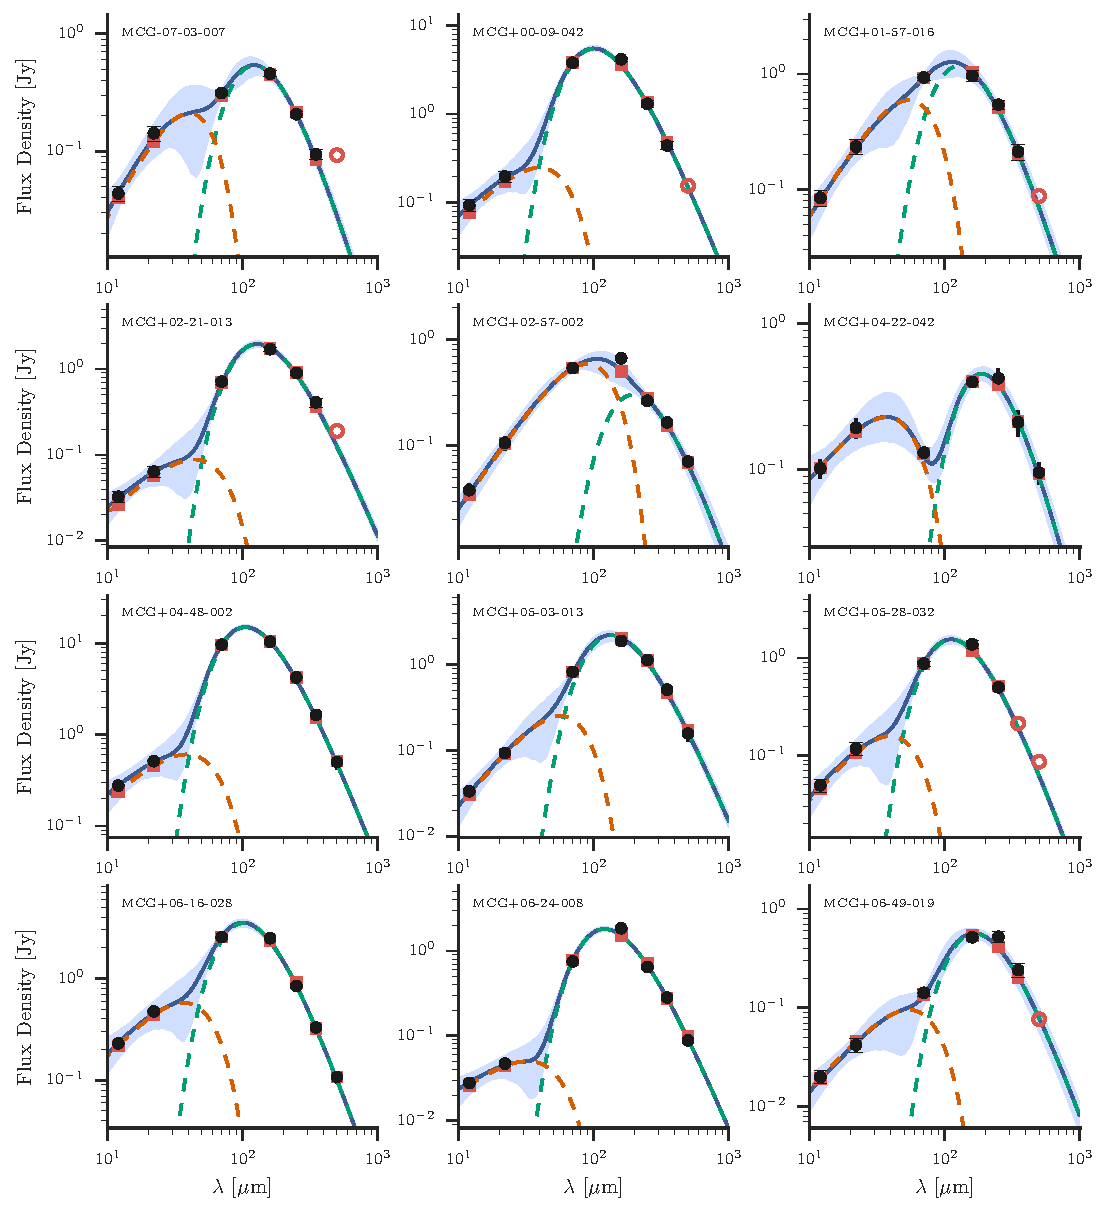
\includegraphics[width=\textwidth]{figures/sedfig15}
\caption{}
\end{figure*}

\begin{figure*}
\centering
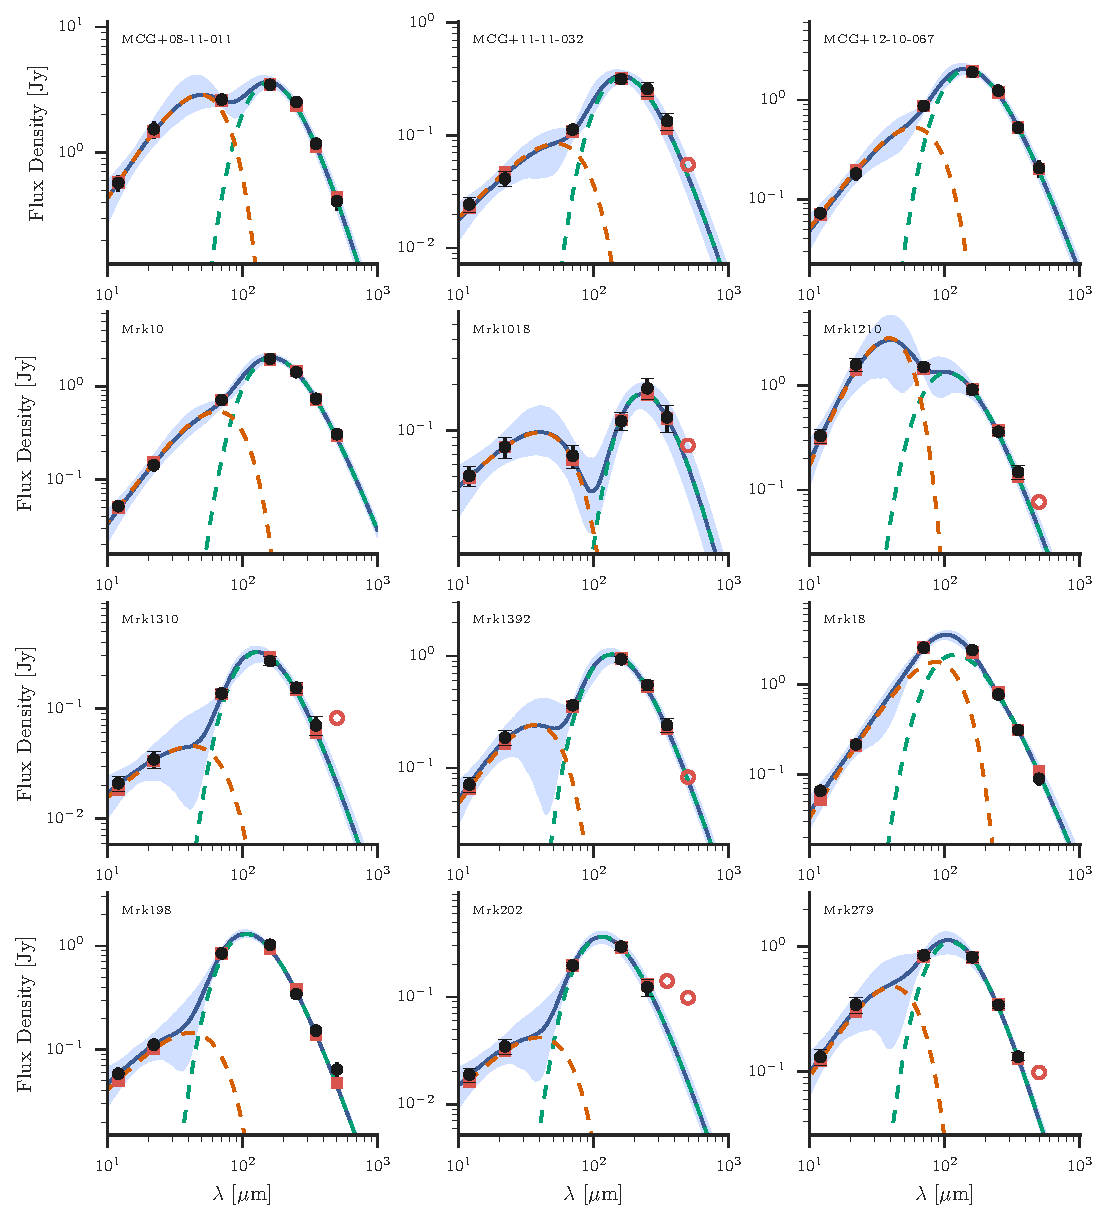
\includegraphics[width=\textwidth]{figures/sedfig16}
\caption{}
\end{figure*}

\begin{figure*}
\centering
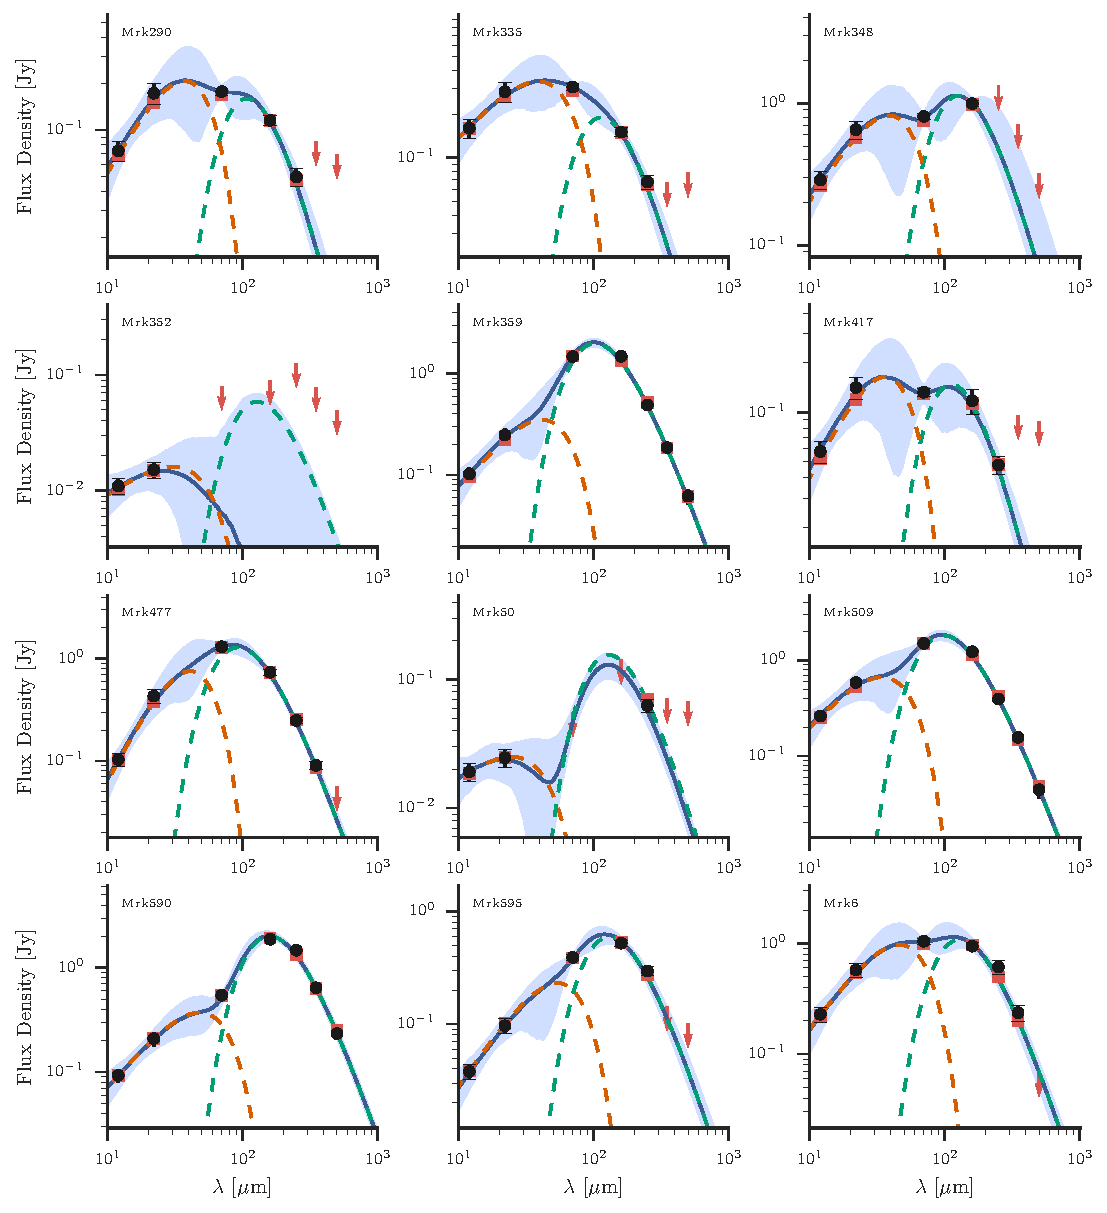
\includegraphics[width=\textwidth]{figures/sedfig17}
\caption{}
\end{figure*}

\begin{figure*}
\centering
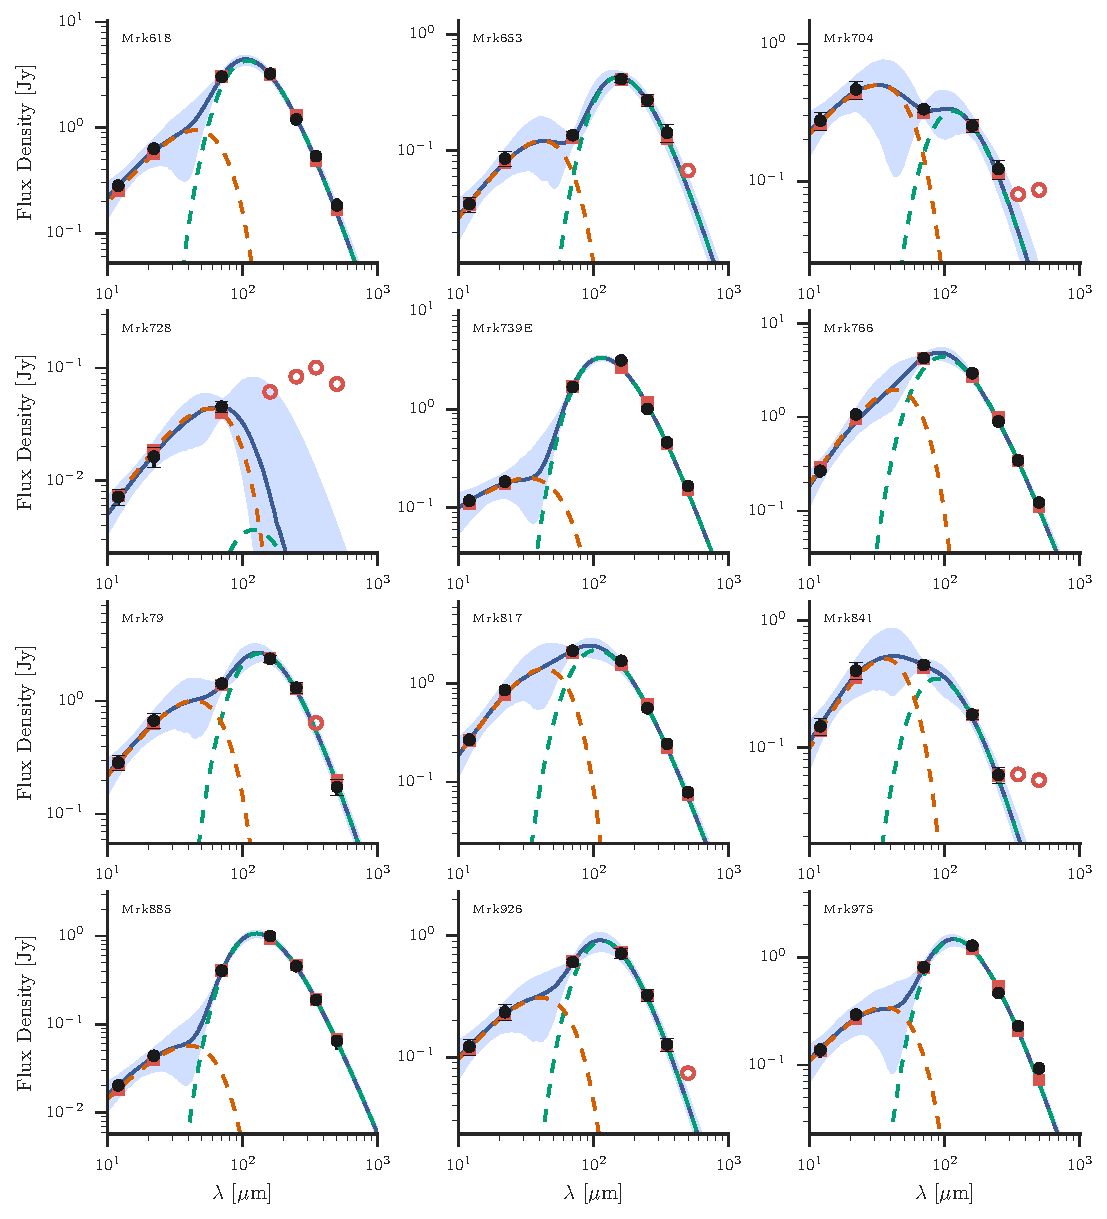
\includegraphics[width=\textwidth]{figures/sedfig18}
\caption{}
\end{figure*}

\begin{figure*}
\centering
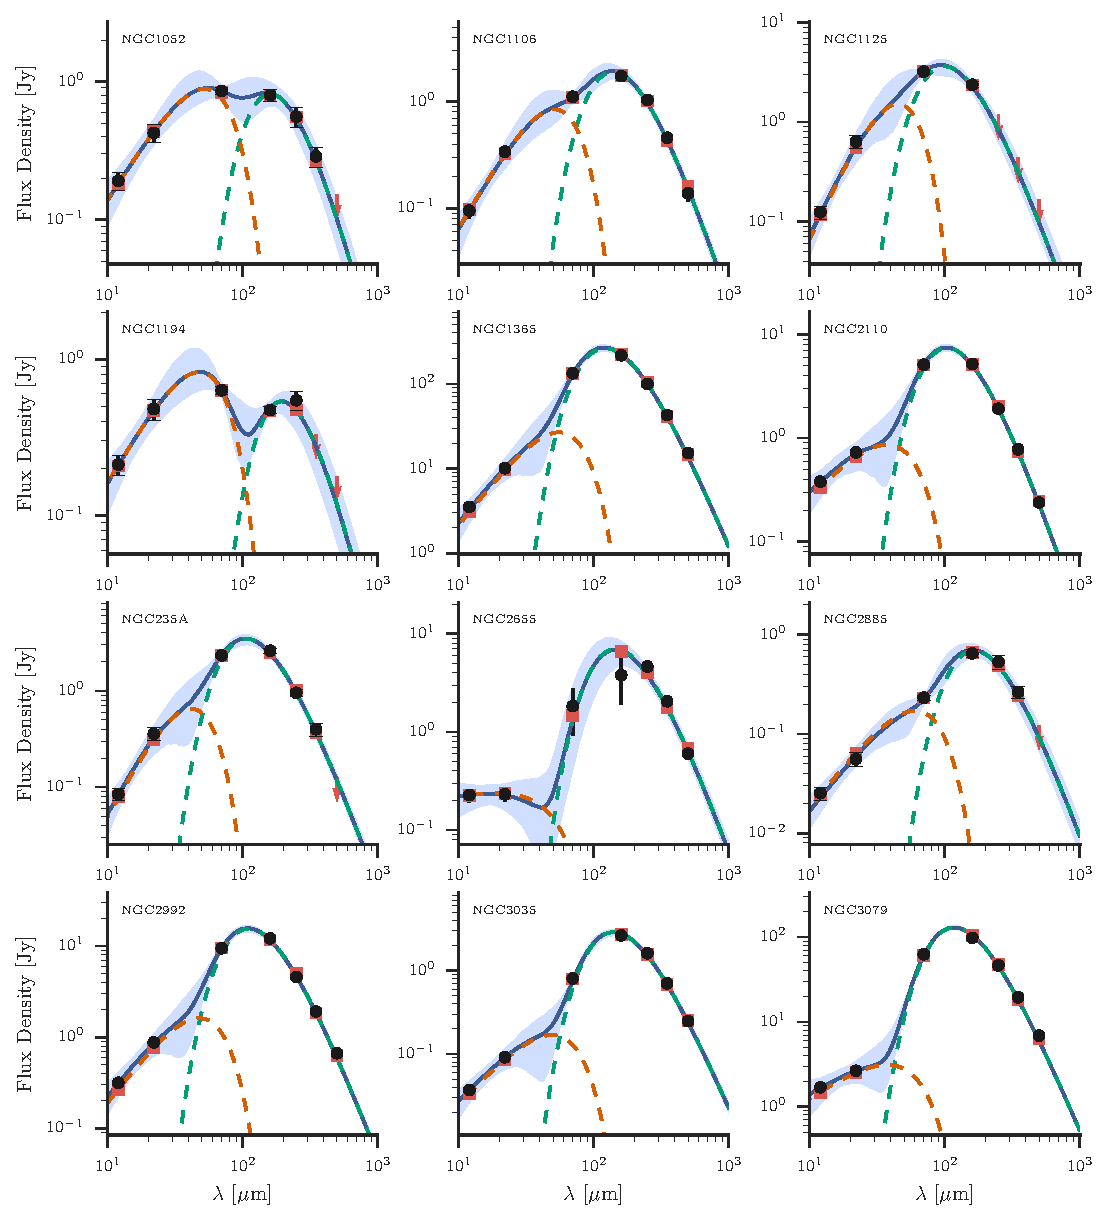
\includegraphics[width=\textwidth]{figures/sedfig19}
\caption{}
\end{figure*}

\begin{figure*}
\centering
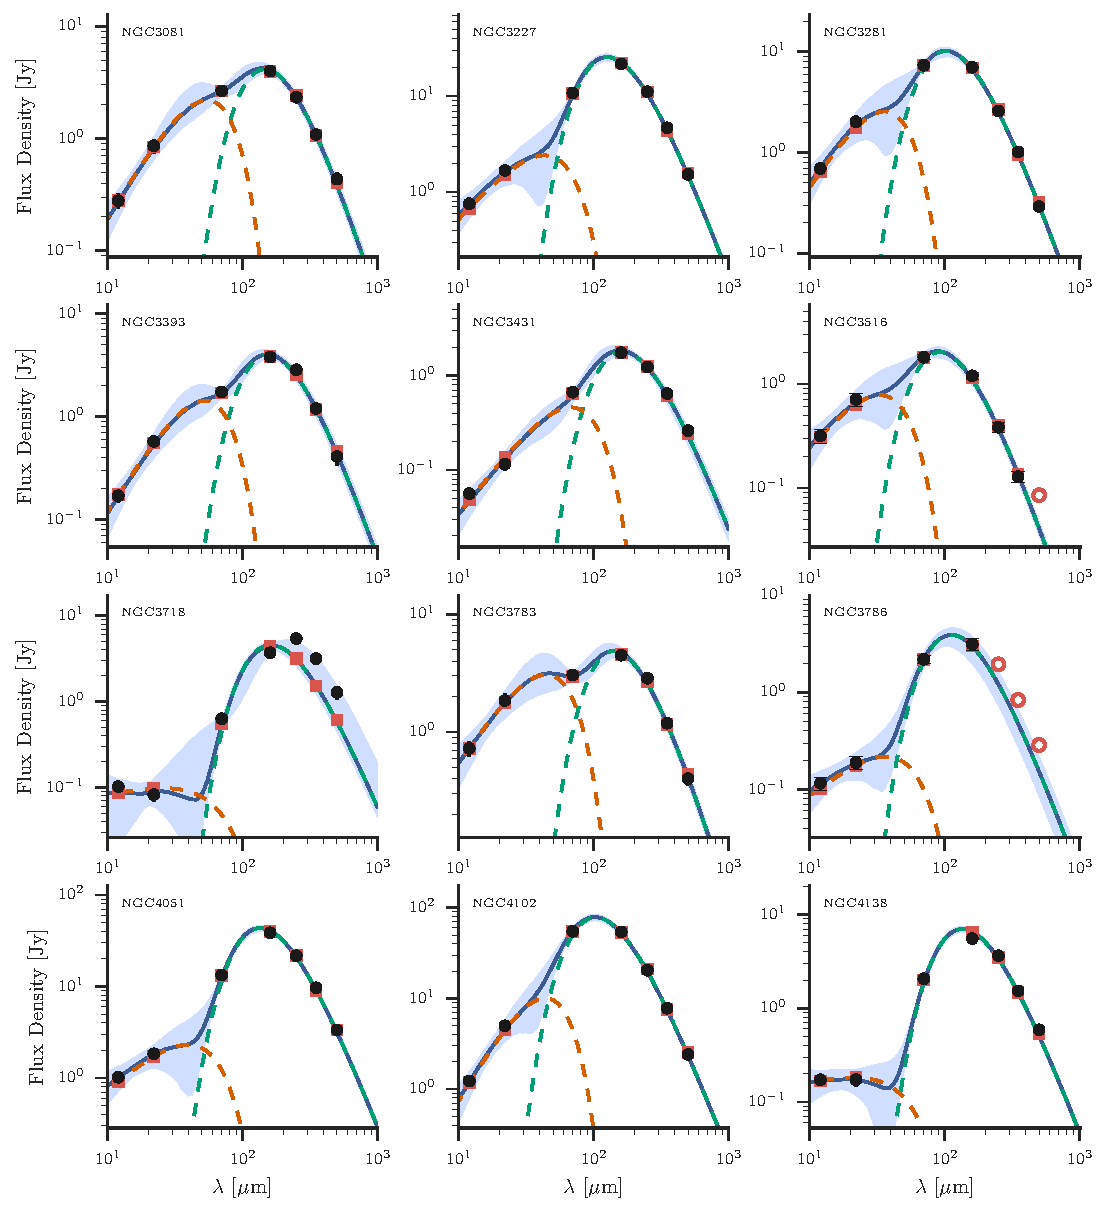
\includegraphics[width=\textwidth]{figures/sedfig20}
\caption{}
\end{figure*}

\begin{figure*}
\centering
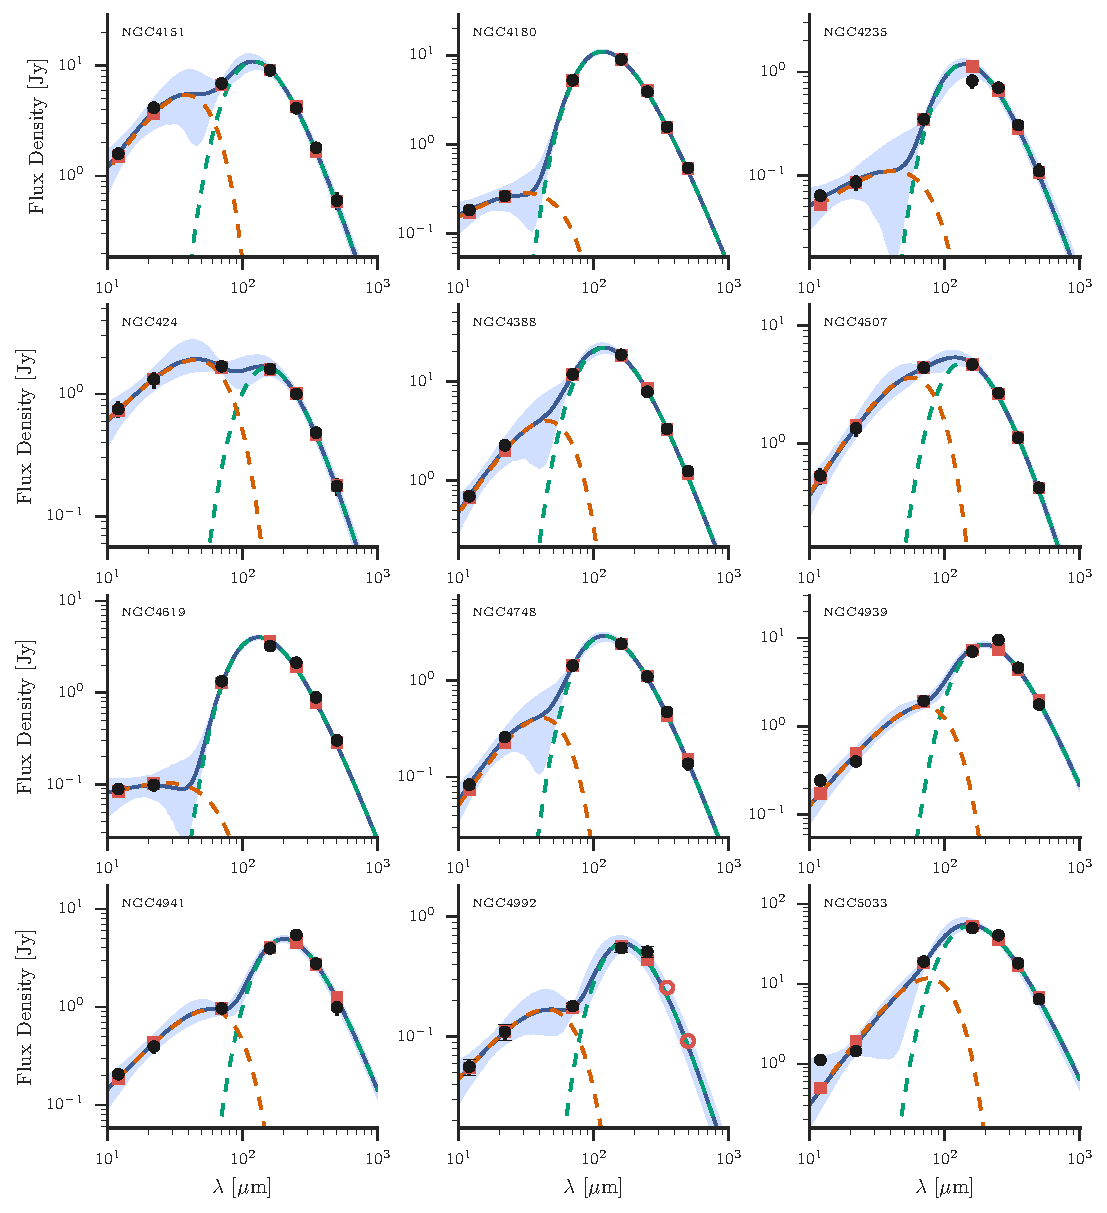
\includegraphics[width=\textwidth]{figures/sedfig21}
\caption{}
\end{figure*}

\begin{figure*}
\centering
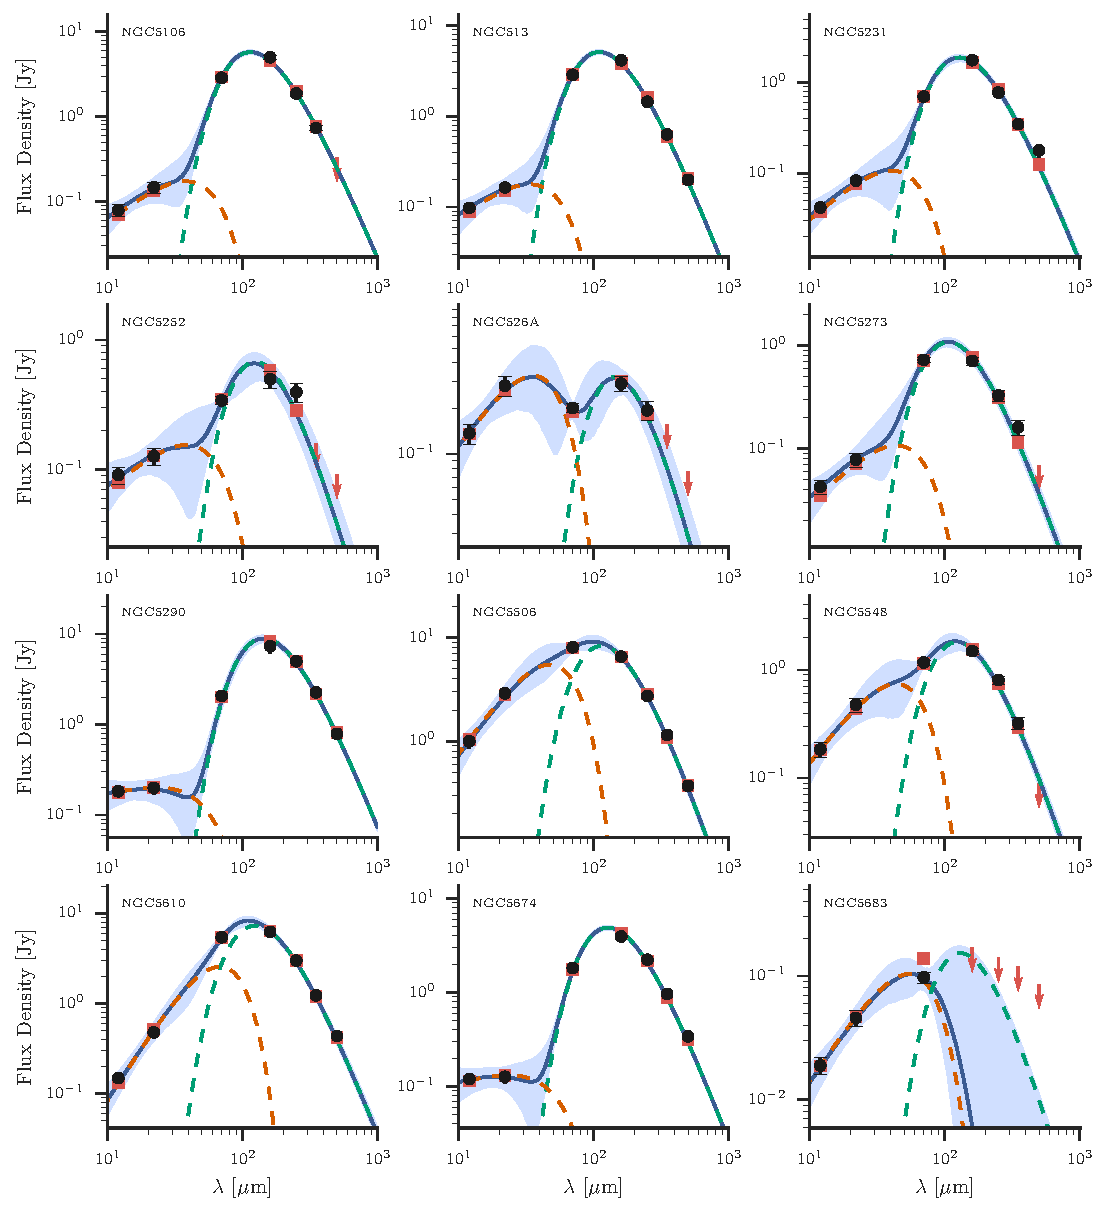
\includegraphics[width=\textwidth]{figures/sedfig22}
\caption{}
\end{figure*}

\begin{figure*}
\centering
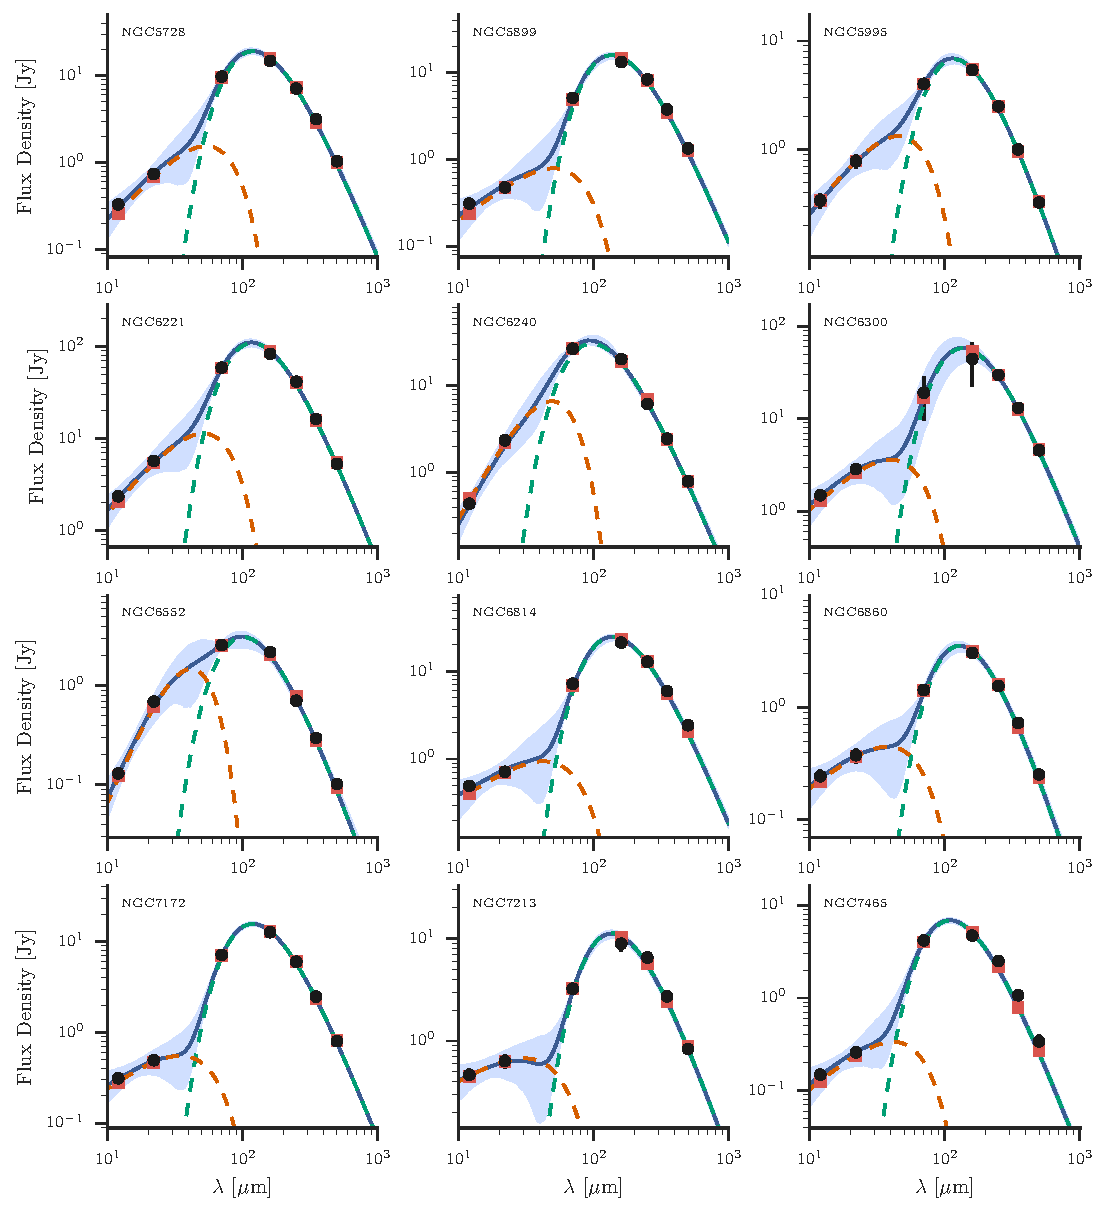
\includegraphics[width=\textwidth]{figures/sedfig23}
\caption{}
\end{figure*}

\begin{figure*}
\centering
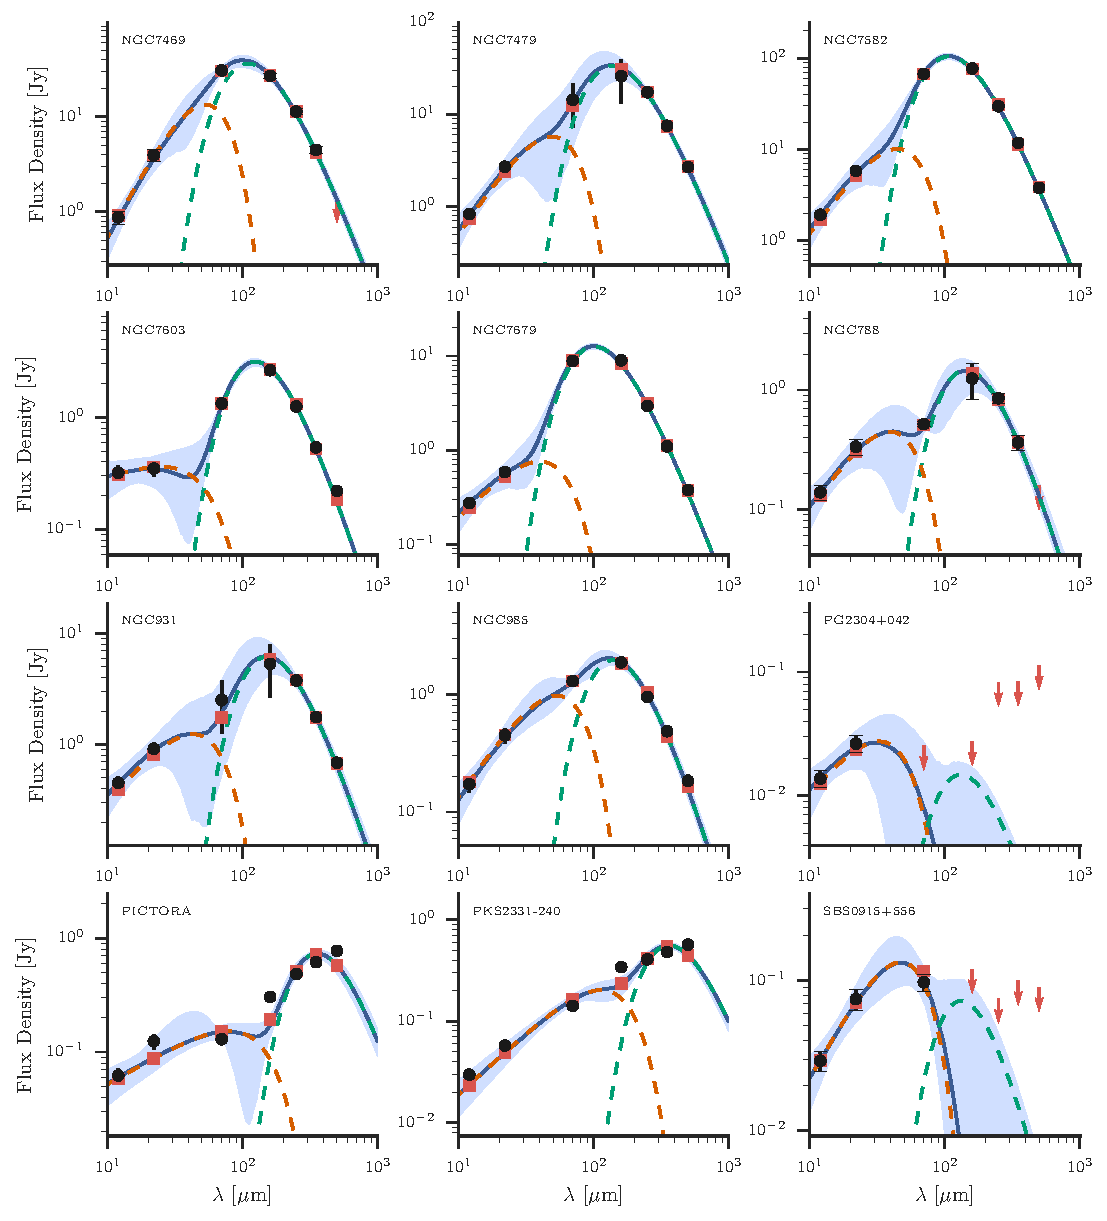
\includegraphics[width=\textwidth]{figures/sedfig24}
\caption{}
\end{figure*}

\begin{figure*}
\centering
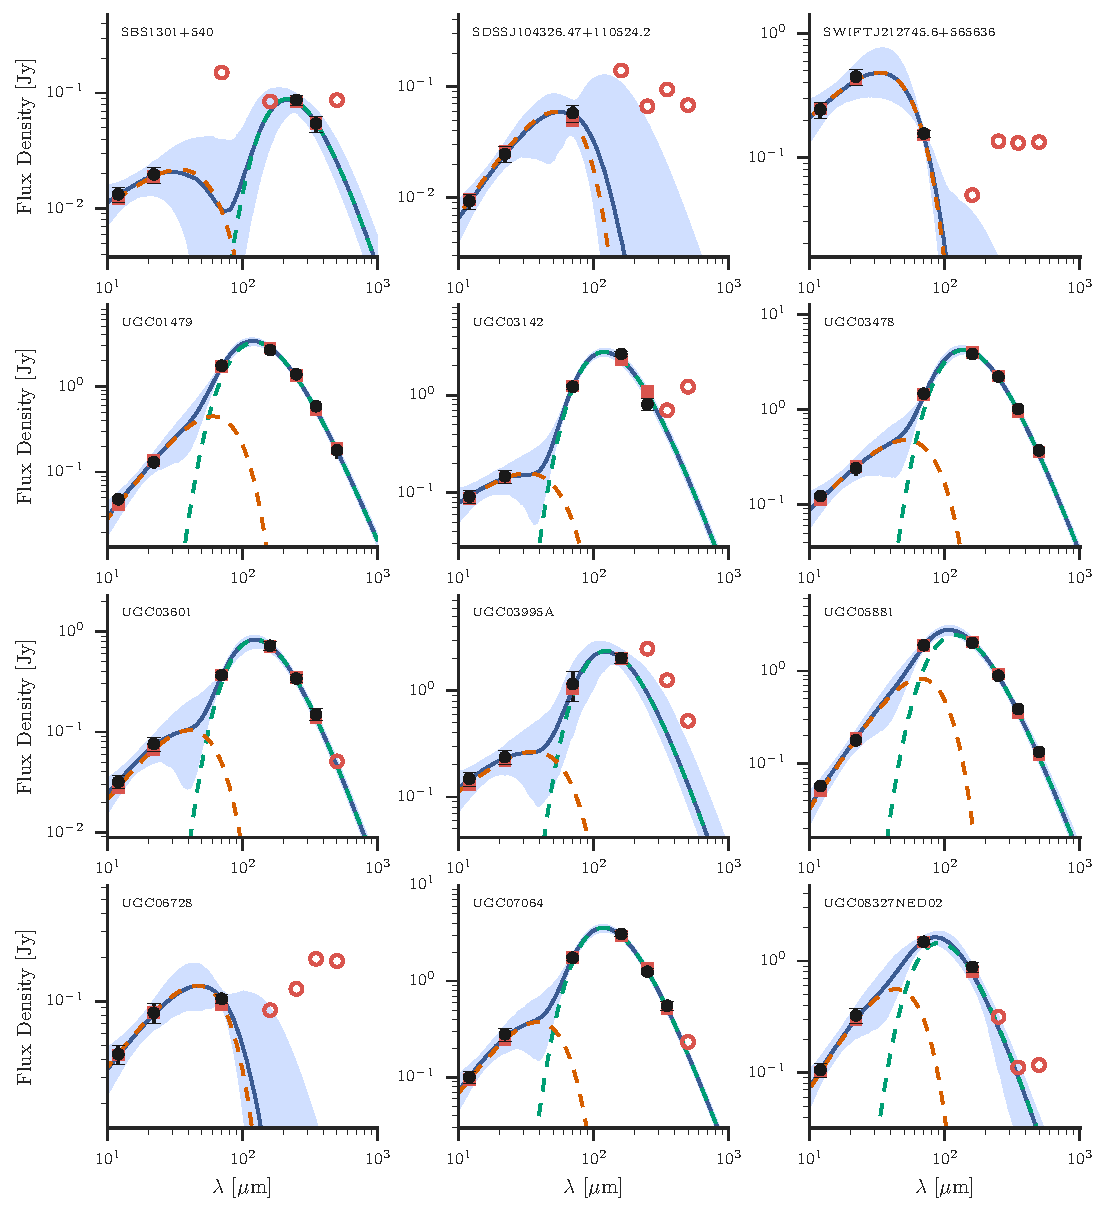
\includegraphics[width=\textwidth]{figures/sedfig25}
\caption{}
\end{figure*}

\begin{figure*}
\centering
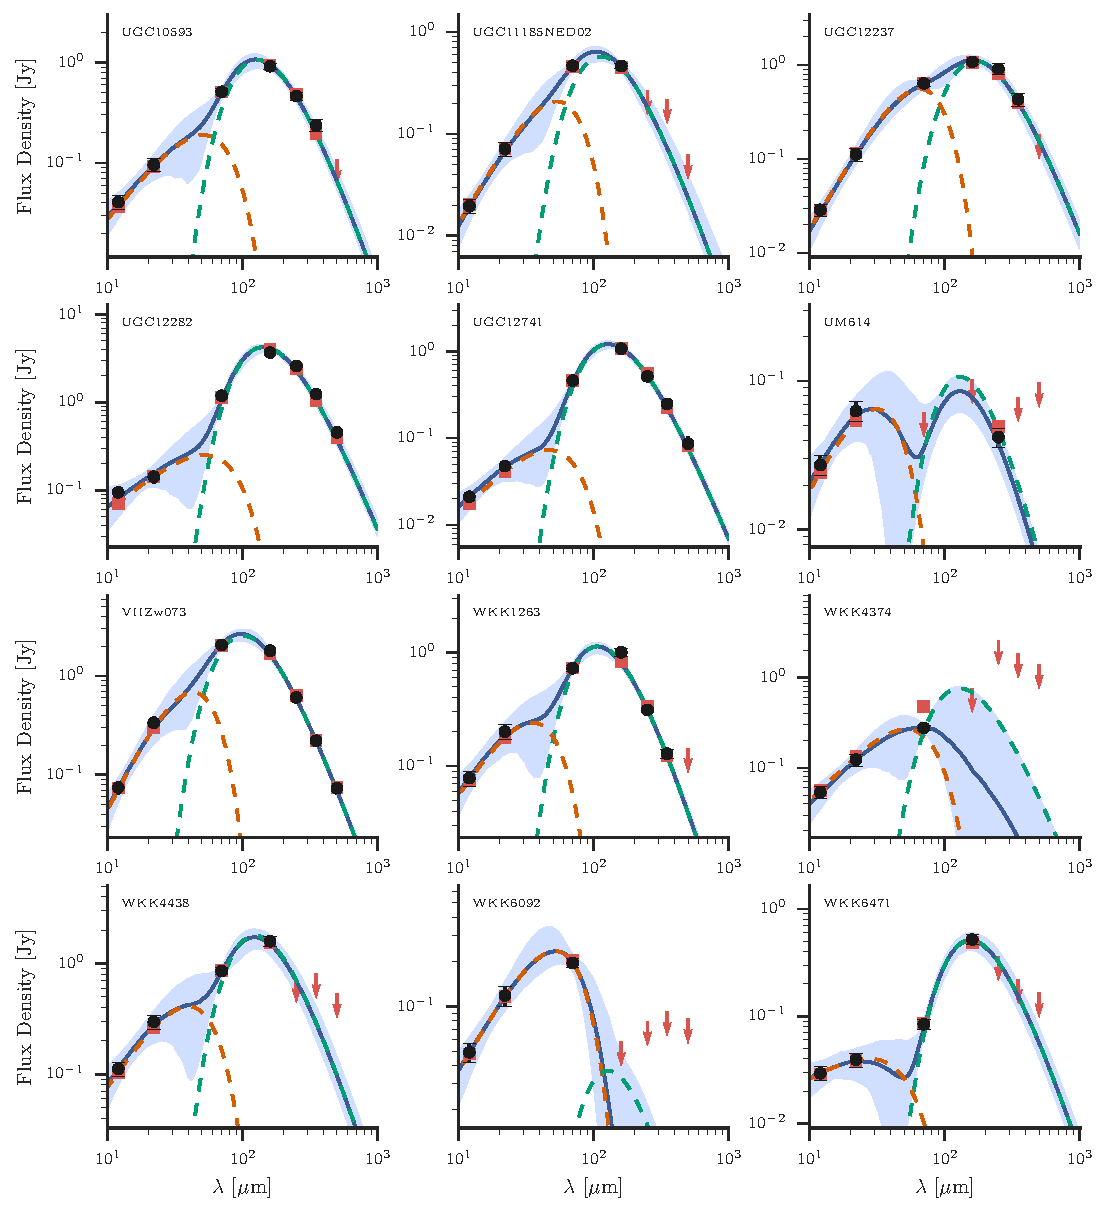
\includegraphics[width=\textwidth]{figures/sedfig26}
\caption{}
\end{figure*}